\documentclass[compress]{beamer}
\usetheme{Warsaw}
\useoutertheme{split}

%%%%%%%%%%%%%%%%%%%%%%%%%%%%%%%%%%%%%%%%%%%%%%%%%%%%%%%%%%%%%%%
% Improvement on the default split theme : added line numbers %
%%%%%%%%%%%%%%%%%%%%%%%%%%%%%%%%%%%%%%%%%%%%%%%%%%%%%%%%%%%%%%%

\setbeamercolor{frametitle}{fg=white}
\setbeamercolor{frametitle right}{fg=white}

\defbeamertemplate*{footline}{mysplit theme}
{%
  \leavevmode%
  \hbox{\begin{beamercolorbox}[wd=.5\paperwidth,ht=2.5ex,dp=1.125ex,leftskip=.3cm plus1fill,rightskip=.3cm]{author in head/foot}%
    \usebeamerfont{author in head/foot}\insertshortauthor
  \end{beamercolorbox}%
  \begin{beamercolorbox}[wd=.4\paperwidth,ht=2.5ex,dp=1.125ex,leftskip=.3cm,rightskip=.3cm plus1fil]{title in head/foot}%
    \usebeamerfont{title in head/foot}\insertshorttitle
  \end{beamercolorbox}}%
    \begin{beamercolorbox}[wd=.1\paperwidth,ht=2.5ex,dp=1.125ex,leftskip=.1cm plus1fill,rightskip=.1cm]{date in head/foot}
      \usebeamerfont{date in head/foot} \insertframenumber{} / \inserttotalframenumber 
    \end{beamercolorbox}
  \vskip0pt%
}

\defbeamertemplate*{headline}{mysplit theme}
{%
  \leavevmode%
  \begin{beamercolorbox}[wd=.45\paperwidth,ht=2.5ex,dp=1.125ex]{section in head/foot}%
    \insertsectionnavigationhorizontal{.4\paperwidth}{\hskip0pt plus1filll}{}%
  \end{beamercolorbox}%
  \begin{beamercolorbox}[wd=.55\paperwidth,ht=2.5ex,dp=1.125ex]{subsection in head/foot}%
    \insertsubsectionnavigationhorizontal{.6\paperwidth}{}{\hskip0pt plus1filll}%
  \end{beamercolorbox}%
}

%%%%%%%%%%%%
% packages %
%%%%%%%%%%%%

\usepackage{scontents}
\makeatletter
\let\verbatimsc\@undefined
\let\endverbatimsc\@undefined
\makeatother
\usepackage{minted}
\newminted{tex}{linenos}
\newenvironment{verbatimsc}
               {\VerbatimEnvironment
                 \begin{minted}[linenos,escapeinside=||]{cpp}}
               {\end{minted}}
\newcommand\highlightCppCode[2]{
  \renewenvironment{verbatimsc}
                   {\VerbatimEnvironment
                     \begin{minted}[linenos,highlightlines={#1},escapeinside=||]{cpp}}
                   {\end{minted}}
  \typestored{#2}
}
\newminted{cpp}{gobble=4,linenos}
\newminted{shell-session}{gobble=4}
\newminted[makefile]{shell-session}{gobble=4}
\newminted{python}{linenos=true,gobble=4}

\usepackage{pgf}
\usepackage{pgffor}
\usepackage{tikz}
\usetikzlibrary{arrows,automata,snakes,shapes}

\usepackage{tcolorbox}

\usepackage[framemethod=TikZ]{mdframed}
\mdfdefinestyle{simplebox}{roundcorner=4pt,linewidth=0,backgroundcolor=blue!50!black,fontcolor=white}

\usepackage{multicol}
\usepackage{tikz-uml}

\usepackage{booktabs}

%%%%%%%%%%%%%%%%%%%
% useful commands %
%%%%%%%%%%%%%%%%%%%
\newcommand{\cpp}{C$^{++}$} 
\newcommand{\deprecated}{\textcolor{red}{\bf Deprecated}}

%%%%%%%%%%%%%%%%%%%%%%%%%%%%%%%
% frametitle with C++ version %
%%%%%%%%%%%%%%%%%%%%%%%%%%%%%%%
% used reverse leet speech for the numbers as a latex command cannot use numbers
% 98 -> gb, 11 -> ii, 14 -> ia, 17 -> it, 20 -> so
\newcommand\frametitlegb[1]{
  \frametitle{#1 \hfill \cpp98}
}
\newcommand\frametitleii[1]{
  \frametitle{#1 \hfill \cpp11}
}
\newcommand\frametitleia[1]{
  \frametitle{#1 \hfill \cpp14}
}
\newcommand\frametitleit[1]{
  \frametitle{#1 \hfill \cpp17}
}
\newcommand\frametitleso[1]{
  \frametitle{#1 \hfill \cpp20}
}

%%%%%%%%%%%%%%%%%%%%%%%%%%%%%%%
% easy class diagrams in tikz %
%%%%%%%%%%%%%%%%%%%%%%%%%%%%%%%

\newcommand\classbox[3][]{
  \def\temp{#3}
  \ifx\temp\empty
    \draw[thick] node (#2) [#1]
         [rectangle,rounded corners,draw] {#2};
  \else
    \draw[thick] node (#2) [#1]
         [rectangle,rounded corners,draw] {
      \begin{tabular}{l}
        \multicolumn{1}{c}{#2} \\
        \hline
        #3
      \end{tabular}
    };
  \fi
}

%%%%%%%%%%%%%%%%%%%%%%%%%%%%%%%%%%%%%%
% easy memory stack diagrams in tikz %
%%%%%%%%%%%%%%%%%%%%%%%%%%%%%%%%%%%%%%

\newcounter{memorystackindex}

\pgfkeys{
  memorystack/.is family,
  memorystack,
  size x/.initial=4cm,
  size y/.initial=.5cm,
  word size/.initial=4,
  nb blocks/.initial=8,
  base address/.initial=12351,
  color/.initial=black,
  addresses/.initial=1
}

\makeatletter

\newcommand\memorystackset[1]{\pgfkeys{memorystack,#1}}
\newcommand\memorystack[1][]{
  \memorystackset{#1,
    size x/.get=\stacksizex,
    size y/.get=\stacksizey,
    word size/.get=\stackwordsize,
    nb blocks/.get=\stacknbblocks,
    base address/.get=\stackbaseaddr,
    color/.get=\stackcolor,
    addresses/.get=\displayaddrs
  }
  \draw[thick,\stackcolor,text=white] node (title)
        at (\stacksizex/2, \stacknbblocks*\stacksizey+.5cm)
        [rectangle,rounded corners,fill=blue!50!black] {Memory layout};
  \setcounter{memorystackindex}{1}
  \draw[thick,\stackcolor] (0,0) rectangle (\stacksizex,\stacknbblocks*\stacksizey);
  \pgfmathsetmacro{\nbbars}{\stacknbblocks-1}
  \pgfmathtruncatemacro\nbbarstrunc{\nbbars}
  \ifnum\nbbarstrunc>0
    \foreach \n in {1,...,\nbbars} {
      \draw[\stackcolor!70] (0,\n*\stacksizey) -- +(\stacksizex,0);
    }
  \fi
  \foreach \n in {1,...,\stacknbblocks} {
    \foreach \p in {1,...,\stackwordsize} {
      \draw node (stack\n-\p)
            at (\stacksizex/\stackwordsize*\p-\stacksizex/\stackwordsize/2,\n*\stacksizey-\stacksizey/2)
            [rectangle,minimum width=\stacksizex,minimum height=\stacksizey] {};
    }
    \ifnum1=\displayaddrs\relax
      \pgfmathparse{\n*\stackwordsize+\stackbaseaddr}
      \pgfmathdectoBase\hexversion{\pgfmathresult}{16}
      \draw node at (\stacksizex,\n*\stacksizey-\stacksizey/2) [right=2pt]
            {0x\hexversion};
    \fi
  }
  \pgfmathsetmacro{\nbseps}{\stackwordsize-1}
  \pgfmathtruncatemacro\nbsepstrunc{\nbseps}
  \ifnum\nbsepstrunc>0
    \foreach \n in {1,...,\nbseps} {
      \draw[\stackcolor!10] (\stacksizex/\stackwordsize*\n,0) -- +(0,\stacknbblocks*\stacksizey);
    }
  \fi
}

\newcommand\memorypushvalue[3]{
  \draw node at (stack#1-#2) {#3};
}

\newcommand\memorypushwidevalue[1]{
  \memorystackset{
    size x/.get=\stacksizex,
    size y/.get=\stacksizey,
  }
  \draw node (content) at (\stacksizex/2,\value{memorystackindex}*\stacksizey-\stacksizey/2) {#1};
  \draw[\stackcolor!80,->] (content) -- (.2cm,\value{memorystackindex}*\stacksizey-\stacksizey/2);
  \draw[\stackcolor!80,->] (content) -- (\stacksizex-.2cm,\value{memorystackindex}*\stacksizey-\stacksizey/2);
  \addtocounter{memorystackindex}{1}
}

\newcommand\memorypushhalfvalue[1]{
  \memorystackset{
    size x/.get=\stacksizex,
    size y/.get=\stacksizey,
  }
  \draw node (content) at (\stacksizex/4,\value{memorystackindex}*\stacksizey-\stacksizey/2) {#1};
  \draw[\stackcolor!80,->] (content) -- (.2cm,\value{memorystackindex}*\stacksizey-\stacksizey/2);
  \draw[\stackcolor!80,->] (content) -- (\stacksizex/2-.2cm,\value{memorystackindex}*\stacksizey-\stacksizey/2);
  \addtocounter{memorystackindex}{1}
}

\newcounter{localcount}
\newcommand\memorypush[1]{
  \memorystackset{
    word size/.get=\stackwordsize,
    nb blocks/.get=\stacknbblocks
  }
  \count@=0
  \setcounter{localcount}{1}
  \@for\v:=#1\do{
    \ifnum\count@<\stackwordsize
      \advance\count@ 1
      \memorypushvalue{\arabic{memorystackindex}}{\arabic{localcount}}{\v}
    \fi
    \addtocounter{localcount}{1}
  }  
  \addtocounter{memorystackindex}{1}
}

\newcommand\memorypushpointer[2][]{
  \memorystackset{
    word size/.get=\stackwordsize,
    base address/.get=\stackbaseaddr
  }
  \pgfmathparse{#2*\stackwordsize+\stackbaseaddr}
  \pgfmathdectoBase\hexaddress{\pgfmathresult}{16}
  \memorypushvalue{\arabic{memorystackindex}}{1}{#1 0x\hexaddress}
  \draw[\stackcolor!80,->] (stack\arabic{memorystackindex}-1.west) .. controls +(left:1) and +(left:1) .. (stack#2-1.west);
  \addtocounter{memorystackindex}{1}
}

\newcommand\memorystruct[3]{
  \memorystackset{
    size y/.get=\stacksizey
  }
  \draw[snake=brace,thick] (-2pt,#1*\stacksizey-\stacksizey) -- (-2pt,#2*\stacksizey)
    node [midway, above, sloped] {#3};
}

\newcommand\memorygoto[1]{
  \setcounter{memorystackindex}{#1}
}
\makeatother

%%%%%%%%%%%%%%%%%%
% Document setup %
%%%%%%%%%%%%%%%%%%

\title{\cpp course}
\author[S. Ponce]{S\'ebastien Ponce \\ \texttt{sebastien.ponce@cern.ch}}
\institute{CERN}
\date{September 2021}
\pgfdeclareimage[height=0.5cm]{cernlogo}{CERN-logo.jpg}
\logo{\pgfuseimage{cernlogo}}

\AtBeginSection[] {
  \begin{frame}<beamer>
    \frametitle{\insertsection}
    \begin{multicols}{2}
      \tableofcontents[sectionstyle=show/shaded,subsectionstyle=show/show/hide]
    \end{multicols}
  \end{frame}
}

\AtBeginSubsection[] {
  \begin{frame}<beamer>
    \frametitle{\insertsubsection}
    \tableofcontents[sectionstyle=show/hide,subsectionstyle=show/shaded/hide]
  \end{frame}
}

%%%%%%%%%%%%%%
% The slides %
%%%%%%%%%%%%%%

\begin{document}

\showboxdepth=\maxdimen
\showboxbreadth=\maxdimen


\begin{frame}
  \titlepage
\end{frame}

\begin{frame}
  \frametitle{Foreword}
  \begin{block}{What this course is not}
    \begin{itemize}
    \item It is not for absolute beginners
    \item It is not for experts
    \item It is not complete at all (would need 3 weeks...)
      \begin{itemize}
      \item although is it already too long for the time we have
      \item \inserttotalframenumber{} slides, \insertpresentationendpage{} pages, 21 exercises...
      \end{itemize}
    \end{itemize}
  \end{block}
  \begin{block}{How I see it}
    \begin{description}
    \item[Adaptative] pick what you want
    \item[Interactive] tell me what to skip/insist on
    \item[Practical] let's spend time on real code
    \end{description}
  \end{block}
  \begin{block}{Where to find latest version ?}
    \begin{itemize}
    \item pdf format at {\small \color{blue} \url{http://cern.ch/sponce/C++Course}}
    \item full sources at {\footnotesize \color{blue} \url{https://github.com/hsf-training/cpluspluscourse}}
    \end{itemize}
  \end{block}
\end{frame}

\begin{frame}
  \frametitle{Outline}
  \begin{multicols}{2}
    \tableofcontents[sectionstyle=show,subsectionstyle=hide]
  \end{multicols}
\end{frame}

\begin{frame}
  \frametitle{Detailed outline}
  %\vspace{-0.5cm}
  \begin{scriptsize}
    \begin{multicols}{3}
      \tableofcontents[sectionstyle=show,subsectionstyle=show]
    \end{multicols}
  \end{scriptsize}
\end{frame}

\section[Intro]{History and goals}

\subsection[Hist]{History}

\begin{frame}
  \frametitle{C/\cpp origins}
  \begin{minipage}{0.4\linewidth}
    \tikzstyle{old}=[ellipse,draw=black,fill=orange!30,thick,inner sep=2pt]
    \tikzstyle{new}=[rectangle,draw=black,fill=green!50,thick,inner sep=2pt]
    \tikzstyle{direct}=[<-,semithick]
    \tikzstyle{transverse}=[<-,dotted,semithick]
    \begin{tikzpicture}[->, node distance=.75cm, font=\tiny, scale=0.9, every node/.style={scale=0.9}]
      \node[old] (Simula)      {Simula};
      \node[left of=Simula,node distance=1.5cm] {1967};
      \node[old] (BCPL) [right of=Simula, node distance=2cm] {BCPL};
      \node[old] (B) [below of=BCPL] {B}
      edge[transverse] (BCPL);
      \node[old] (KandRC) [below of=B] {K and R C}
      edge[transverse] (B);
      \node[left of=KandRC,node distance=3.5cm] {1978};
      \node[old] (ClassicC) [below of=KandRC] {Classic C}
      edge[direct] (KandRC);
      \node[old] (CwithClasses) [below of=Simula,node distance=3cm] {C with Classes}
      edge[transverse] (Simula)
      edge[transverse] (BCPL)
      edge[direct] (ClassicC);
      \node[left of=CwithClasses,node distance=1.5cm] {1980};
      \node[old] (EarlyC++) [below of=CwithClasses] {Early \cpp}
      edge[direct] (CwithClasses);
      \node[left of=EarlyC++,node distance=1.5cm] {1985};
      \node[old] (C89) [below of=ClassicC,node distance=2.25cm] {C89}
      edge[direct] (ClassicC)
      edge[transverse] (CwithClasses);
      \node[old] (ARMC++) [below of=EarlyC++] {ARM \cpp}
      edge[direct] (EarlyC++)
      edge[transverse] (C89);
      \node[left of=ARMC++,node distance=1.5cm] {1989};
      \node[old] (C++98) [below of=ARMC++] {\cpp98}
      edge[direct] (ARMC++)
      edge[transverse] (C89);
      \node[old] (C99) [below of=C89] {C99}
      edge[direct] (C89)
      edge[transverse] (ARMC++);
      \node[left of=C++98,node distance=1.5cm] {1998};
      \node[new] (C++11) [below of=C++98] {\cpp11}
      edge[direct] (C++98)
      edge[transverse] (C99);
      \node[left of=C++11,node distance=1.5cm] {2011};
      \node[new] (C11) [below of=C99] {C11}
      edge[direct] (C99)
      edge[transverse] (C++98);
      \node[new] (C18) [below of=C11,node distance=1.8cm] {C18}
      edge[direct] (C11);
      \node[new] (C++14) [below of=C++11] {\cpp14}
      edge[direct] (C++11);
      \node[left of=C++14,node distance=1.5cm] {2014};
      \node[new] (C++17) [below of=C++14] {\cpp17}
      edge[direct] (C++14);
      \node[left of=C++17,node distance=1.5cm] {2017};
      \node[new] (C++20) [below of=C++17] {\cpp20}
      edge[direct] (C++17);
      \node[left of=C++20,node distance=1.5cm] {2020};
    \end{tikzpicture}
  \end{minipage}
  \begin{minipage}{0.57\linewidth}
    \begin{tabular}{cc}
      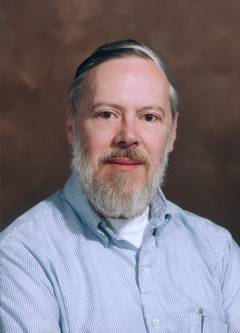
\includegraphics[height=2.5cm]{ritchie.jpeg} & 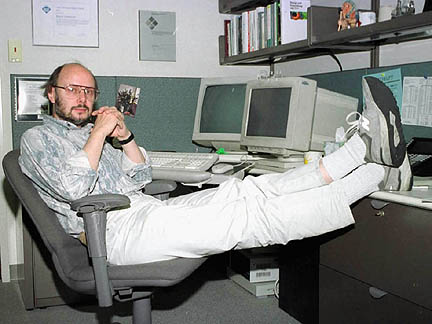
\includegraphics[height=2.5cm]{BjarneStroustrup.jpg} \\[-1ex]
      \tiny{C inventor} & \tiny{\cpp inventor} \\[-1ex]
      \scriptsize{Dennis M. Ritchie} & \scriptsize{Bjarne Stroustrup} \\
    \end{tabular}
    \begin{itemize}
      {\footnotesize
      \item Both C and \cpp are born in Bell Labs
      \item \cpp {\it almost} embeds C
      \item C and \cpp are still under development
      \item We will discuss all \cpp specs but \cpp20
      \item Each slide will be marked with first spec introducting the feature
      }
    \end{itemize}
  \end{minipage}
\end{frame}

\begin{frame}
  \frametitle{\cpp11, \cpp14, \cpp17, \cpp20...}
  \begin{block}{status}
    \begin{itemize}
    \item A new \cpp specification every 3 years
      \begin{itemize}
      \item \cpp20 is ready, officially published by ISO in December 2020
      \end{itemize}
    \item Bringing each time a lot of goodies
    \end{itemize}
  \end{block}
  \pause
  \begin{block}{How to use \cpp XX features}
    \begin{multicols}{2}
      \begin{itemize}
      \item Use a compatible compiler
      \item add -std=c++xx to compilation flags
      \item e.g. -std=c++17
      \end{itemize}
      \vfill
      \columnbreak
      \begin{table}[h!]
        \begin{center}
          \begin{tabular}{c|c|c}
            \textbf{\cpp} & \textbf{gcc} & \textbf{clang}\\
            \hline
            11 & $\geq$4.8 & $\geq$3.3\\
            14 & $\geq$4.9 & $\geq$3.4\\
            17 & $\geq$7.3 & $\geq$5\\
            20 & $>$10  & $>$10 \\
          \end{tabular}
          \caption{Minimum versions of gcc and clang for a given \cpp version}
        \end{center}
      \end{table}
    \end{multicols}
  \end{block}
\end{frame}

\subsection[Use]{Why we use it ?}

\begin{frame}
  \frametitle{Why is \cpp our language of choice ?}
  \begin{block}{Adapted to large projects}
    \begin{itemize}
    \item strongly typed
    \item object oriented
    \item widely used (and taught)
    \item many available libraries
    \end{itemize}
  \end{block}
  \pause
  \begin{block}{Fast}
    \begin{itemize}
    \item compiled (unlike Java or C\#)
    \item allows to go close to hardware when needed
    \end{itemize}
  \end{block}
  \pause
  \begin{alertblock}{What we get}
    \begin{itemize}
    \item the most powerful language
    \item the most complicated one
    \item the most error prone ?
    \end{itemize}
  \end{alertblock}
\end{frame}

\section[Basics]{Langage basics (C and \cpp)}

\subsection[Core]{Core syntax and types}

\begin{frame}[fragile]
  \frametitle{Hello World}
  \begin{cppcode}
    #include <iostream>

    // This is a function
    void print(int i) {
      std::cout << "Hello, world " << i << std::endl;
    }

    int main(int argc, char** argv) {
      int n = 3;
      for (int i = 0; i < n; i++) {
        print(i);
      }
      return 0;
    }
  \end{cppcode}
\end{frame}

\begin{frame}[fragile]
  \frametitle{Comments}
  \begin{cppcode}
    // simple comment for integer declaration
    int i;

    /* multiline comment
     * in case we need to say more
     */
    double d;

    /**
     * Best choice : doxygen compatible comments
     * \fn bool isOdd(int i)
     * \brief checks whether i is odd
     * \param i input
     * \return true if i is odd, otherwise false
     */
    bool isOdd(int i);
  \end{cppcode}
\end{frame}

\begin{frame}[fragile]
  \frametitle{Basic types(1)}
  \begin{cppcode}
    bool b = true;            // boolean, true or false
    
    char c = 'a';             // 8 bits ASCII char
    char* s = "a C string";   // array of chars ended by \0
    string t = "a C++ string";// class provided by the STL

    char c = -3;              // 8 bits signed integer
    unsigned char c = 4;      // 8 bits unsigned integer

    short int s = -444;       // 16 bits signed integer
    unsigned short s = 444;   // 16 bits unsigned integer
    short s = -444;           // int is optional
  \end{cppcode}
\end{frame}
\begin{frame}[fragile]
  \frametitle{Basic types(2)}
  \begin{cppcode}
    int i = -123456;          // 32 bits signed integer
    unsigned int i = 1234567; // 32 bits signed integer

    long l = 0L               // 32 or 64 bits (ptr size)
    unsigned long l = 0UL;    // 32 or 64 bits (ptr size)

    long long ll = 0LL;       // 64 bits signed integer
    unsigned long long l = 0ULL; // 64 bits unsigned integer

    float f = 1.23;           // 32 (23+7+1) bits float
    double d = 1.23E34;       // 64 (52+11+1) bits float
  \end{cppcode}
\end{frame}

\begin{frame}[fragile]
  \frametitle{Portable numeric types}
  \alert{One needs to include specific header}
  \begin{cppcode}
    #include <cstdint>
    
    int8_t c = -3;     // 8 bits, replaces char
    uint8_t c = 4;     // 8 bits, replaces unsigned char

    int16_t s = -444;  // 16 bits, replaced short
    uint16_t s = 444;  // 16 bits, replaced unsigned short

    int32_t s = -0674; // 32 bits, replaced int
    uint32_t s = 0674; // 32 bits, replaced unsigned int

    int64_t s = -0x1bc;// 64 bits, replaced long long
    uint64_t s = 0x1bc;// 64 bits, replaced unsigned long long
    \end{cppcode}
\end{frame}

\subsection[Pointers]{Arrays and Pointers}

\begin{frame}[fragile]
  \frametitle{Static arrays}
  \begin{cppcode}
    int ai[4] = {1,2,3,4};
    int ai[] = {1,2,3,4};  // identical
    
    char ac[3] = {'a','b','c'};   // char array
    char ac[4] = "abc";           // valid C string
    char ac[4] = {'a','b','c',0}; // same valid string
    
    int i = ai[2];  // i = 3
    char c = ac[8]; // at best garbage, may segfault
    int i = ai[4];  // also garbage !
  \end{cppcode}
\end{frame}

\begin{frame}[fragile]
  \frametitle{Pointers}
  \begin{multicols}{2}
    \begin{cppcode*}{gobble=2}
      int i = 4;
      int *pi = &i;
      int j = *pi + 1;
      
      int ai[] = {1,2,3};
      int *pai = ai;
      int *paj = pai + 1;
      int k = *paj + 1;
      
      int *pak = k; // not compiling
      int *pak = (int*)k;
      int l = *pak; // seg fault !
    \end{cppcode*}
    \onslide<2->{
      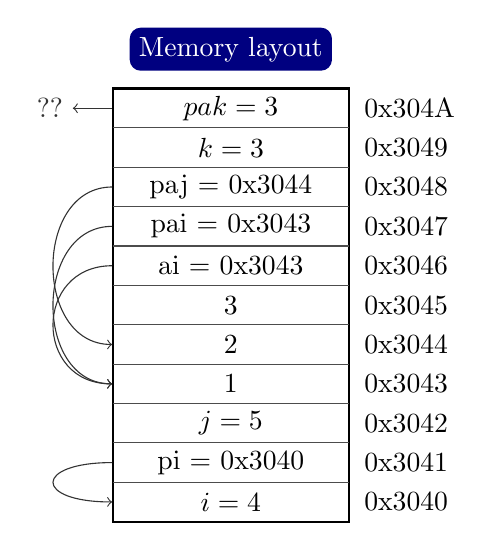
\begin{tikzpicture}
        \memorystack[size x=3cm,word size=1,nb blocks=11]
        \onslide<3-> {\memorypush{$i = 4$}}
        \onslide<4-> {\memorypushpointer[pi =]{1}}
        \onslide<5-> {\memorypush{$j = 5$}}
        \onslide<6-> {\memorypush{$1$}}
        \onslide<6-> {\memorypush{$2$}}
        \onslide<6-> {\memorypush{$3$}}
        \onslide<6-> {\memorypushpointer[ai =]{4}}
        \onslide<7-> {\memorypushpointer[pai =]{4}}
        \onslide<8-> {\memorypushpointer[paj =]{5}}
        \onslide<9-> {\memorypush{$k = 3$}}
        \onslide<10-> {\memorypush{$pak = 3$}}
        \onslide<10-> {\draw[\stackcolor!80,->] (stack11-1.west) -- +(-0.5cm,0)
          node [anchor=east] {??};}
      \end{tikzpicture}
    }
  \end{multicols}
\end{frame}

\begin{frame}[fragile]
  \frametitle{Dynamic Arrays}
  \begin{cppcode}
    #include <cstdlib>
    #include <cstring>

    int *bad;    // pointer to random address
    int *ai = 0; // better. Can be tested

    // allocate array of 10 ints (not initialized)
    ai = (int*) malloc(10*sizeof(int));
    // and set them to 0
    memset(ai, 0, 10*sizeof(int));

    // Both in one go
    ai = (int*) calloc(10, sizeof(int));
    
    // liberate memory
    free(ai);
  \end{cppcode}
\end{frame}

\subsection{Operators}

\begin{frame}[fragile]
  \frametitle{Operators(1)}
  \begin{block}{Binary \& Assignment Operators}
    \begin{cppcode*}{linenos=false}
      int i = 1 + 4 - 2;  // 3
      i *= 3;             // 9
      i /= 2;             // 4
      i = 23 % i;         // modulo => 3
    \end{cppcode*}
  \end{block}
  \pause
  \begin{block}{Increment / Decrement \uncover<3->{\hfill \alert{\bf Use wisely}}}
    \begin{cppcode*}{linenos=false}
      int i = 0; i++; // i = 1
      int j = ++i;    // i = 2, j = 2
      int k = i++;    // i = 3, k = 2
      int l = --i;    // i = 2, l = 2
      int m = i--;    // i = 1, m = 2
    \end{cppcode*}
  \end{block}
\end{frame}

\begin{frame}[fragile]
  \frametitle{Operators(2)}
  \begin{block}{Bitwise and Assignment Operators}
    \begin{cppcode*}{linenos=false}
      int i = 0xee & 0x55;  // 0x44
      i |= 0xee;            // 0xee
      i ^= 0x55;            // 0xbb
      int j = ~0xee;        // 0xffffff11
      int k = 0x1f << 3;    // 0x78
      int l = 0x1f >> 2;    // 0x7
    \end{cppcode*}
  \end{block}
  \pause
  \begin{block}{Boolean Operators}
    \begin{cppcode*}{linenos=false}
      bool a = true;
      bool b = false;
      bool c = a && b;    // false
      bool d = a || b;    // true
      bool e = !d;        // false
    \end{cppcode*}
  \end{block}
\end{frame}

\begin{frame}[fragile]
  \frametitle{Operators(3)}
  \begin{block}{Comparison Operators}
    \begin{cppcode*}{linenos=false}
      bool a = (3 == 3);  // true
      bool b = (3 != 3);  // false
      bool c = (4 < 4);   // false
      bool d = (4 <= 4);  // true
      bool e = (4 > 4);   // false
      bool f = (4 >= 4);  // true
    \end{cppcode*}
  \end{block}
  \pause
  \begin{block}{Precedences \uncover<3->{\hfill \alert{\bf Don't use}\uncover<4->{\color{green} \bf\ - use parenthesis}}}
    \begin{cppcode*}{linenos=false}
      c &= 1+(++b)|(a--)*4%5^7; // ???
    \end{cppcode*}
  \end{block}
\end{frame}

\subsection[Compound]{Compound data types}

\begin{frame}[fragile]
  \frametitle{struct}
  \begin{mdframed}[style=simplebox]
    \center ``members'' grouped together under one name
  \end{mdframed}
  \begin{multicols}{2}
    \begin{cppcode*}{gobble=2}
      struct Individual {
        unsigned char age;
        float weight;
      };

      Individual student;
      student.age = 25;
      student.weight = 78.5;

      Individual teacher = {
        .age = 45,
        .weight=67
      };
    \end{cppcode*}
    \pause
    \columnbreak
    \null \vfill
    \hspace{-1.5cm}
    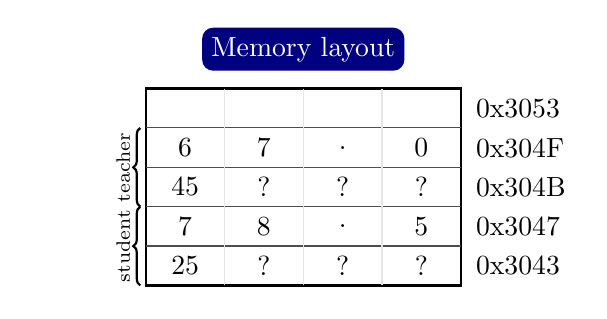
\begin{tikzpicture}
      \memorystack[nb blocks=5]
      \onslide<3-> {
        \memorypush{25,?,?,?}
        \memorypush{7,8,.,5}
        \memorystruct{1}{2}{\scriptsize student}
      }
      \onslide<4-> {
        \memorypush{45,?,?,?}
        \memorypush{6,7,.,0}
        \memorystruct{3}{4}{\scriptsize teacher}
      }
    \end{tikzpicture}
    \vfill \null
  \end{multicols}
\end{frame}

\begin{frame}[fragile]
  \frametitle{union}
  \begin{mdframed}[style=simplebox]
    \center ``members'' packed together at same memory location
  \end{mdframed}
  \begin{multicols}{2}
    \begin{cppcode*}{gobble=2}
      union Duration {
        int seconds;
        short hours;
        char days;
      };

      Duration d1, d2, d3;
      d1.seconds = 259200;
      d2.hours = 72;
      d3.days = 3;
      d1.days = 3; // d1.seconds overwritten
      int a = d1.seconds; // d1.seconds is garbage
    \end{cppcode*}
    \pause
    \columnbreak
    \null \vfill
    \onslide<2->{
      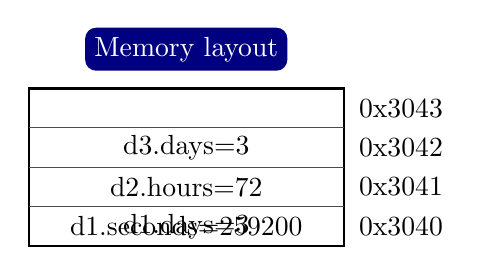
\begin{tikzpicture}
        \memorystack[word size=1,nb blocks=4]
        \visible<3-5>{\memorypush{d1.seconds=259200}}
        \onslide<4->{\memorypush{d2.hours=72}}
        \onslide<5->{\memorypush{d3.days=3}}
        \memorygoto{1}
        \onslide<6->{\memorypush{d1.days=3}}
      \end{tikzpicture}
    }
    \vfill \null
  \end{multicols}
\end{frame}

\begin{frame}[fragile]
  \frametitle{Enums and typedefs}
  \begin{multicols}{2}
    \begin{cppcode*}{gobble=2}
      enum VehicleType {
        BIKE,  // 0
        CAR,   // 1
        BUS,   // 2
      };
      VehicleType t = CAR;
      
      typedef uint64_t myint;
      myint toto = 17;
    \end{cppcode*}
    \columnbreak
    \begin{cppcode*}{gobble=2}
      enum VehicleType {
        BIKE = 3,
        CAR = 5,
        BUS = 7,
      };
      VehicleType t2 = BUS;
    \end{cppcode*}
  \end{multicols}
\end{frame}


\begin{frame}[fragile]
  \frametitle{More sensible example}
  \begin{multicols}{2}
    \begin{cppcode*}{gobble=2}
      enum ShapeType {
        CIRCLE,
        RECTANGLE
      };
      
      struct Rectangle {
        float width;
        float height;
      };
    \end{cppcode*}
    \columnbreak
    \pause
    \begin{cppcode*}{gobble=2,firstnumber=10}
      struct Shape {
        ShapeType type;
        union { 
          float radius;
          Rectangle rect;
        };
      };
    \end{cppcode*}
  \end{multicols}
  \pause
  \begin{multicols}{2}
    \begin{cppcode*}{gobble=2,firstnumber=17}
      Shape s;
      s.type = CIRCLE;
      s.radius = 3.4;
      
    \end{cppcode*}
    \columnbreak
    \begin{cppcode*}{gobble=2,firstnumber=20}
      Shape t;
      t.type = RECTANGLE;
      t.rect.width = 3;
      t.rect.height = 4;
    \end{cppcode*}
  \end{multicols}
\end{frame}

\subsection[$f()$]{Functions}

\begin{frame}[fragile]
  \frametitle{Functions}
  \begin{multicols}{2}
    \begin{cppcode*}{gobble=2}
      // with return type
      int square(int a) {
        return a * a;
      }

      // multiple parameters
      int mult(int a,
               int b) {
        return a*b;
      }
    \end{cppcode*}
    \columnbreak
    \begin{cppcode*}{gobble=2,firstnumber=11}
      // no parameter
      void hello() {
        printf("Hello World");
      }

      // no return
      void log(char* msg) {
        printf("%s", msg);
      }
    \end{cppcode*}
  \end{multicols}
\end{frame}

\begin{frame}[fragile]
  \frametitle{Parameter are passed by value}
  \begin{multicols}{2}
    \begin{cppcode*}{gobble=2}
      struct BigStruct {...};
      BigStruct s;
      
      // parameter by value
      void printBS(BigStruct p) {
        ...
      }
      printBS(s); // replication
      
      // parameter by pointer
      void printBSp(BigStruct *q) {
        ...
      }
      printBSp(&s); // not replication
    \end{cppcode*}
    \columnbreak
    \null \vfill
    \onslide<2->{
      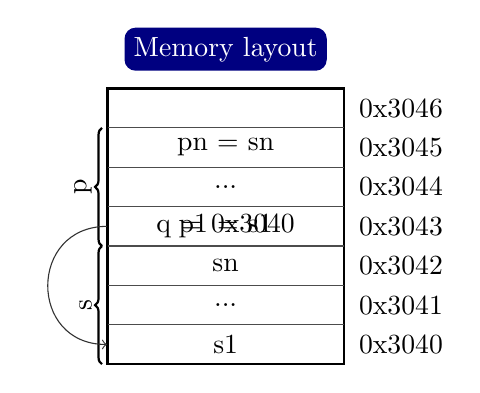
\begin{tikzpicture}
        \memorystack[word size=1, nb blocks=7, size x=3cm]
        \onslide<3-> {
          \memorypush{s1}
          \memorypush{...}
          \memorypush{sn}
          \memorystruct{1}{3}{s}
        }
        \onslide<4> {
          \memorypush{p1 = s1}
          \memorypush{...}
          \memorypush{pn = sn}
          \memorystruct{4}{6}{p}
        }
        \memorygoto{4}
        \onslide<6> {
          \memorypushpointer[q =]{1}
        }
      \end{tikzpicture}
    }
    \vfill \null
  \end{multicols}
\end{frame}

\begin{frame}[fragile]
  \frametitle{Parameter are passed by value}
  \begin{multicols}{2}
    \begin{cppcode*}{gobble=2}
      struct SmallStruct {int a};
      SmallStruct s = {.a = 1};
      
      void changeSS(SmallStruct p) {
        p.a = 2;
      }
      changeSS(s);
      // s.a = 1
      
      void changeSS2(SmallStruct *q) {
        q->a = 2;  // i.e. (*q).a
      }
      changeSS2(s);
      // s.a = 2
    \end{cppcode*}
    \columnbreak
    \null \vfill
    \onslide<2->{
      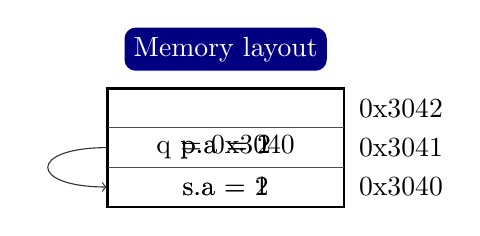
\begin{tikzpicture}
        \memorystack[word size=1, nb blocks=3, size x=3cm]
        \onslide<3-7> {
          \memorypush{s.a = 1}
        }
        \onslide<4> {
          \memorypush{p.a = 1}
        }
        \memorygoto{2}
        \onslide<5> {
          \memorypush{p.a = 2}
        }
        \memorygoto{2}
        \onslide<7-> {
          \memorypushpointer[q =]{1}
        }
        \memorygoto{1}
        \onslide<8> {
          \memorypush{s.a = 2}
        }
      \end{tikzpicture}
    }
    \vfill \null
  \end{multicols}
\end{frame}

\subsection[Control]{Control instructions}

\begin{frame}[fragile]
  \frametitle{Control instructions : if}
  \begin{block}{if syntax}
    \begin{cppcode*}{linenos=false}
      if (condition1) {
        Instructions1;
      } else if (condition2) {
        Instructions2;
      } else {
        Instructions3;
      } 
    \end{cppcode*}
    \vspace{-0.5cm}
    \begin{itemize}
      \item {\it else} and {\it else if} part are optional
      \item {\it else if} part can be repeated
      \item braces are optional if there is a single instruction
    \end{itemize}
  \end{block}
\end{frame}

\begin{frame}[fragile]
  \frametitle{Control instructions : if}
  \begin{exampleblock}{Practical example}
    \begin{cppcode*}{linenos=false}
      int collatz(int a) {
        if (a <= 0) {
          std::cout << "not supported";
          return 0;
        } else if (a == 1) {
          return 1;
        } else if (a%2 == 0) {
          return collatz(a/2);
        } else {
          return collatz(3*a+1);
        }
      }
    \end{cppcode*}
  \end{exampleblock}
\end{frame}

\begin{frame}[fragile]
  \frametitle{Control instructions : conditional operator}
  \begin{block}{Syntax}
    \begin{cppcode*}{linenos=false}
      test ? expression1 : expression2;
    \end{cppcode*}
    \vspace{-0.3cm}
    \begin{itemize}
      \item if test is {\it true} expression1 is returned
      \item else expression 2 is returned
    \end{itemize}
  \end{block}
  \pause
  \begin{exampleblock}{Practical example}
    \begin{cppcode*}{linenos=false}
      int collatz(int a) {
        return a==1 ? 1 : collatz(a%2 ? 3*a+1 : a/2);
      }
    \end{cppcode*}
  \end{exampleblock}
  \pause
  \begin{alertblock}{Do not abuse}
    explicit ifs are easier to read \\
    to be used only when obvious and not nested
  \end{alertblock}
\end{frame}

\begin{frame}[fragile]
  \frametitle{Control instructions : switch}
  \begin{block}{Syntax}
    \begin{cppcode*}{gobble=2,linenos=false}
      switch(identifier) {
        case c1 : instructions1; break;
        case c2 : instructions2; break;
        case c3 : instructions3; break;
        ...
        default : instructiond; break;
      }
    \end{cppcode*}
    \vspace{-0.5cm}
    \begin{itemize}
      \item {\it break} is not mandatory but...
      \item cases are entry points, not independant pieces
      \item execution carries on with the next case if no {\it break} is present !
      \item {\it default} may be omitted
    \end{itemize}
  \end{block}
  \pause
  \begin{alertblock}{Use break}
    Do not try to make use of non breaking cases
  \end{alertblock}
\end{frame}

\begin{frame}[fragile]
  \frametitle{Control instructions : switch}
  \begin{exampleblock}{Practical example}
    \begin{cppcode*}{linenos=false}
      enum Lang { FRENCH, GERMAN, ENGLISH, OTHER };
      ...
      switch (language) {
      case FRENCH:
        printf("Bonjour");
        break;
      case GERMAN:
        printf("Guten tag");
        break;
      case ENGLISH:
        printf("Good morning");
        break;
      default:
        printf("I do not talk your langage");
      }
    \end{cppcode*}
  \end{exampleblock}
\end{frame}

\begin{frame}[fragile]
  \frametitle{Control instructions : for loop}
  \begin{block}{for loop syntax}
    \begin{cppcode*}{linenos=false}
      for(initializations; condition; increments) {
        instructions;
      }
    \end{cppcode*}
    \vspace{-0.5cm}
    \begin{itemize}
      \item initializations and increments are comma separated
      \item initializations can contain declarations
      \item braces are optional if there is a single instruction
    \end{itemize}
  \end{block}
  \pause
  \begin{exampleblock}{Practical example}
    \begin{cppcode*}{linenos=false}
      for(int i = 0, j = 0 ; i < 10 ; i++, j = i*i) {
        std::cout << i << "^2 is " << j << "\n";
      }
    \end{cppcode*}
  \end{exampleblock}
  \pause
  \begin{alertblock}{Do not abuse the syntax}
    The for statement should fit in 1-3 lines
  \end{alertblock}
\end{frame}

\begin{frame}[fragile]
  \frametitle{Control instructions : while loop}
  \begin{block}{while loop syntax}
    \begin{cppcode*}{linenos=false}
      while(condition) {
        instructions;
      }
      do {
        Instructions;
      } while(condition);
    \end{cppcode*}
    \vspace{-0.3cm}
    \begin{itemize}
      \item braces are optional if there is a single instruction
    \end{itemize}
  \end{block}
  \pause
  \begin{exampleblock}{Practical example}
    \begin{cppcode*}{linenos=false}
      while (n != 1)
        if (0 == n%2) n /= 2; 
        else n = 3 * n + 1;
    \end{cppcode*}
  \end{exampleblock}
\end{frame}

\begin{frame}[fragile]
  \frametitle{Control instructions : commands}
  \begin{block}{control commands}
    \begin{description}
    \item[break] goes out of the loop
    \item[continue] goes immediately to next iteration
    \item[return] goes out of current function
    \end{description}
  \end{block}
  \pause
  \begin{exampleblock}{Practical example}
    \begin{cppcode*}{linenos=false}
      while (1) {
        if (n == 1) break;
        if (0 == n%2) {
          std::cout << n << "\n";
          n /= 2;
          continue;
        }
        n = 3 * n + 1;
      }
    \end{cppcode*}
  \end{exampleblock}
\end{frame}

\subsection[Headers]{Headers and interfaces}

\begin{frame}[fragile]
  \frametitle{Headers and interfaces}
  \begin{block}{Interface}
    Set of declarations defining some functionnality
    \begin{itemize}
    \item defined in a ``header file''
    \item no implementation defined
    \end{itemize}
  \end{block}
  \begin{block}{Header : Hello.hpp}
    \begin{cppcode*}{linenos=false}
      void printHello();
    \end{cppcode*}
  \end{block}
  \begin{block}{Usage : myfile.cpp}
    \begin{cppcode*}{linenos=false}
      #include "hello.hpp"
      int main() {
        printHello();
      }
    \end{cppcode*}  
  \end{block}
\end{frame}

\begin{frame}[fragile]
  \frametitle{Preprocessor}
  \begin{cppcode}
    // file inclusion
    #include "hello.hpp"
    // macros
    #define MY_GOLDEN_NUMBER 1746
    // compile time decision
    #ifdef USE64BITS
      typedef uint64_t myint;
    #else
      typedef uint32_t myint;
    #endif
  \end{cppcode}
  \pause
  \begin{block}{Use only in very restricted cases}
    \begin{itemize}
    \item include of headers
    \item hardcoded constants {\scriptsize (should this happen at all ?)}
    \item portability necessity
    \end{itemize}
  \end{block}
\end{frame}

\section[OO]{Object orientation}

\subsection[Objects]{Objects and Classes}

\begin{frame}[fragile]
  \frametitle{What are classes and objects}
  \begin{block}{Classes}
    structs on steroids
    \begin{itemize}
    \item with inheritance
    \item including methods
    \end{itemize}
  \end{block}
  \begin{block}{Objects}
    instances of classes
  \end{block}
  \begin{block}{A class encapsulates a concept}
    \begin{itemize}
    \item shows an interface
    \item provides its implementation
      \begin{itemize}
      \item status, properties
      \item possible interactions
      \item construction and destruction
      \end{itemize}    
    \end{itemize}    
  \end{block}
\end{frame}


\begin{frame}[fragile]
  \frametitle{My First Class}
  \begin{multicols}{2}
    \begin{cppcode*}{gobble=2}
      struct MyFirstClass {
        int a;
        void squareA() {
          a *= a;
        };
        int sum(int b) {
          return a + b;
        };
      };

      MyFirstClass myObj;
      myObj.a = 2;

      // let's square a
      myObj.squareA();
    \end{cppcode*}
    \columnbreak
    \center
    \null \vfill
    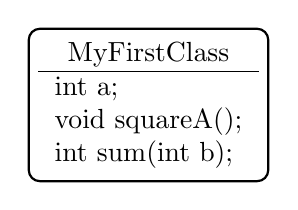
\begin{tikzpicture}
      \classbox{MyFirstClass}{
        int a; \\
        void squareA(); \\
        int sum(int b);
      }
    \end{tikzpicture}
    \vfill \null
  \end{multicols}
\end{frame}

\begin{frame}[fragile]
  \frametitle{Separating the interface}
  \begin{block}{Header : MyFirstClass.hpp}
    \begin{cppcode*}{linenos=false}
      struct MyFirstClass {
        int a;
        void squareA();
        int sum(int b)();
      };
    \end{cppcode*}
  \end{block}
  \begin{block}{Implementation : MyFirstClass.cpp}
    \begin{cppcode*}{linenos=false}
      #include "MyFirstClass.hpp"
      void MyFirstClass::squareA() {
        a *= a;
      };
      void MyFirstClass::sum(int b) {
        return a + b;
      };
    \end{cppcode*}
  \end{block}
\end{frame}

\begin{frame}[fragile]
  \frametitle{A word on namespaces}
  \begin{itemize}
  \item Namespaces allow to segment your code to avoid name clashes
  \item They can be embedded to create hierarchies (separator is '::')
  \end{itemize}
  \begin{multicols}{2}
    \begin{cppcode*}{gobble=2}
      int a;
      namespace n {
        int a;   // no clash
      }      
      namespace p {
        int a;   // no clash
        namespace inner {
          int a; // no clash
        }
      }
      int f() {
        n::a = 2;
      }
    \end{cppcode*}
    \columnbreak
    \begin{cppcode*}{gobble=2,firstnumber=14}
      namespace p {
        int f() {
          p::a = 2;
          a = 2;  //same as above
          p::inner::a = 4;
          inner::a = 4;
          n::a = 5;
        }
      }
      using namespace p::inner;
      int g() {
        a = 3; // using p::inner
      }
  \end{cppcode*}
  \end{multicols}
\end{frame}

\begin{frame}[fragile]
  \frametitle{Implementing methods}
  \begin{block}{Standard practice}
    \begin{itemize}
    \item usually in .cpp, outside of class declaration
    \item using the class name as namespace
    \item when reference to the object is needed, use {\it this} keyword
    \end{itemize}
  \end{block}
  \begin{cppcode}
    void MyFirstClass::squareA() {
      a *= a;
    };

    int MyFirstClass::sum(int b) {
      int a = 0; // do not do that !
      a += this->a;
      a += b;
      return a;
    };
  \end{cppcode}
\end{frame}

\begin{frame}[fragile]
  \frametitle{Method overloading}
  \begin{block}{The rules in \cpp}
    \begin{itemize}
    \item overloading is authorized and welcome
    \item signature is part of the method identity
    \item but not the return code
    \end{itemize}
  \end{block}
  \begin{cppcode}
    struct MyFirstClass {
      int a;
      int sum(int b);
      int sum(int b, int c);
    }

    int MyFirstClass::sum(int b) { return a + b; };

    int MyFirstClass::sum(int b, int c) {
      return a + b + c;
    };
  \end{cppcode}
\end{frame}

\subsection{Inheritance}

\begin{frame}[fragile]
  \frametitle{First inheritance}
  \begin{multicols}{2}
    \begin{cppcode*}{gobble=2}
      struct MyFirstClass {
        int a;
        void squareA() { a *= a; };
      };
      struct MySecondClass :
        MyFirstClass {
        int b;
        int sum() { return a + b; };
      };

      MySecondClass myObj2;
      myObj2.a = 2;
      myObj2.b = 5;
      myObj2.squareA();
      int i = myObj2.sum(); // i = 9
    \end{cppcode*}
    \columnbreak
    \center
    \null \vfill
    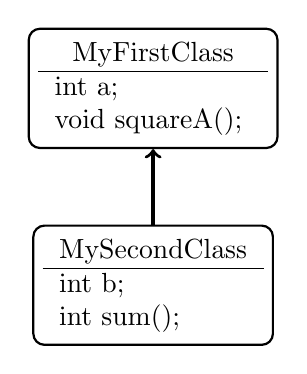
\begin{tikzpicture}[node distance=2.5cm]
      \classbox{MyFirstClass}{
        int a; \\
        void squareA();
      }
      \classbox[below of=MyFirstClass]{MySecondClass}{
        int b; \\
        int sum();
      }
      \draw[very thick,->] (MySecondClass)--(MyFirstClass);
    \end{tikzpicture}
    \vfill \null
  \end{multicols}
\end{frame}

\begin{frame}[fragile]
  \frametitle{Managing access to class members}
  \begin{block}{{\it public} / {\it private} keywords}
    \begin{description}
      \item[private] allows access only within the class
      \item[public] allows access from anywhere
    \end{description}
    \begin{itemize}
      \item Default is {\it private}
      \item A {\it struct} is a {\it class} where all members are public
    \end{itemize}
  \end{block}
  \pause
  \begin{multicols}{2}
    \begin{cppcode*}{gobble=2}
      class MyFirstClass {
      public:
        void setA(int a);
        int getA();
        void squareA();
      private:
        int a;
      }
    \end{cppcode*}
    \columnbreak
    \begin{cppcode*}{gobble=2,firstnumber=9}
      MyFirstClass obj;
      obj.a = 5;   // error !
      obj.setA(5); // ok
      obj.squareA();
      int b = obj.getA();
    \end{cppcode*}
    \pause
    \begin{tcolorbox}[left=0mm,right=0mm,top=0mm,bottom=0mm,colback=red!5!white,colframe=red!75!black]
      This breaks MySecondClass !
    \end{tcolorbox}
  \end{multicols}
\end{frame}

\begin{frame}[fragile]
  \frametitle{Managing access to class members(2)}
  \begin{block}{Solution is {\it protected} keyword}
    Gives access to classes inheriting from base class
  \end{block}
  \begin{multicols}{2}
    \begin{cppcode*}{gobble=2}
      class MyFirstClass {
      public:
        void setA(int a);
        int getA();
        void squareA();
      protected:
        int a;
      }
    \end{cppcode*}
    \columnbreak
    \begin{cppcode*}{gobble=2,firstnumber=13}
      class MySecondClass :
        public MyFirstClass {
      public:
        int sum() {
          return a + b;
        };
      private:
        int b;
      }
    \end{cppcode*}
  \end{multicols}
\end{frame}

\begin{frame}[fragile]
  \frametitle{Managing inheritance privacy}
  \begin{block}{Inheritance can be public, protected or private}
    The influences the privacy of inherited members for external code.\\
    The code of the class itself is not affected
    \begin{description}
    \item[public] privacy of inherited members remains unchanged
    \item[protected] inherited public members are seen as protected
    \item[private] all inherited members are seen as private \\
      this is the default if nothing is specified
    \end{description}
  \end{block}
  \pause
  \begin{block}{Net result for external code}
    \begin{itemize}
    \item only public members of public inheritance are accessible
    \end{itemize}
  \end{block}
  \begin{block}{Net result for grand child code}
    \begin{itemize}
    \item only public and protected members of public and protected parents are accessible
    \end{itemize}
  \end{block}
\end{frame}

\begin{frame}[fragile]
  \frametitle{Managing inheritance privacy - public}
  \begin{multicols}{2}
    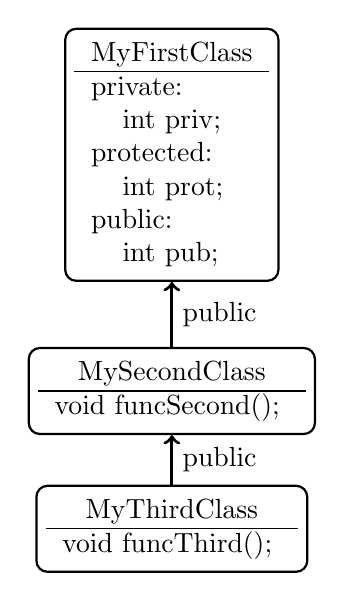
\begin{tikzpicture}[node distance=3cm]
      \classbox{MyFirstClass}{
      private: \\
        \hspace{0.4cm}int priv; \\
      protected: \\
        \hspace{0.4cm}int prot; \\
      public: \\
        \hspace{0.4cm}int pub;
      }
      \classbox[below of=MyFirstClass]{MySecondClass}{
        void funcSecond();
      }
      \classbox[below of=MySecondClass,node distance=1.75cm]{MyThirdClass}{
        void funcThird();
      }
      \draw[very thick,->] (MySecondClass)--(MyFirstClass) node[midway,right] {public};
      \draw[very thick,->] (MyThirdClass)--(MySecondClass) node[midway,right] {public};
    \end{tikzpicture}
    \columnbreak
    \begin{cppcode*}{gobble=2}
      void funcSecond() {
        int a = priv;   // Error
        int b = prot;   // OK
        int c = pub;    // OK
      }
      void funcThird() {
        int a = priv;   // Error
        int b = prot;   // OK
        int c = pub;    // OK
      }
      void extFunc(MyThirdClass t) {
        int a = t.priv; // Error
        int b = t.prot; // Error
        int c = t.pub;  // OK
      }
    \end{cppcode*}
  \end{multicols}
\end{frame}

\begin{frame}[fragile]
  \frametitle{Managing inheritance privacy - protected}
  \begin{multicols}{2}
    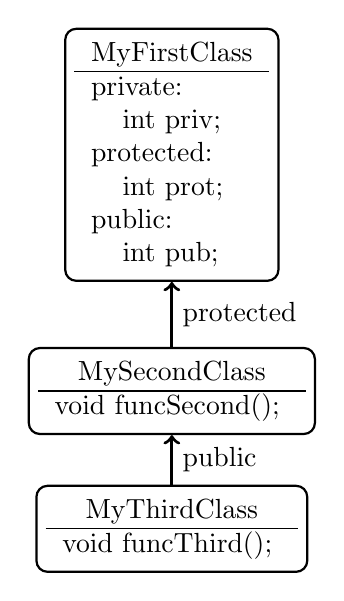
\begin{tikzpicture}[node distance=3cm]
      \classbox{MyFirstClass}{
      private: \\
        \hspace{0.4cm}int priv; \\
      protected: \\
        \hspace{0.4cm}int prot; \\
      public: \\
        \hspace{0.4cm}int pub;
      }
      \classbox[below of=MyFirstClass]{MySecondClass}{
        void funcSecond();
      }
      \classbox[below of=MySecondClass,node distance=1.75cm]{MyThirdClass}{
        void funcThird();
      }
      \draw[very thick,->] (MySecondClass)--(MyFirstClass) node[midway,right] {protected};
      \draw[very thick,->] (MyThirdClass)--(MySecondClass) node[midway,right] {public};
    \end{tikzpicture}
    \columnbreak
    \begin{cppcode*}{gobble=2}
      void funcSecond() {
        int a = priv;   // Error
        int b = prot;   // OK
        int c = pub;    // OK
      }
      void funcThird() {
        int a = priv;   // Error
        int b = prot;   // OK
        int c = pub;    // OK
      }
      void extFunc(MyThirdClass t) {
        int a = t.priv; // Error
        int b = t.prot; // Error
        int c = t.pub;  // Error
      }
    \end{cppcode*}
  \end{multicols}
\end{frame}

\begin{frame}[fragile]
  \frametitle{Managing inheritance privacy - private}
  \begin{multicols}{2}
    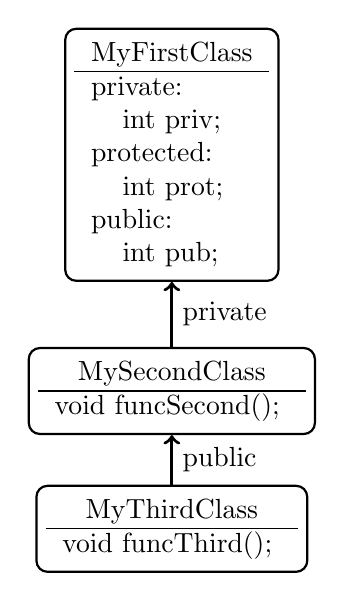
\begin{tikzpicture}[node distance=3cm]
      \classbox{MyFirstClass}{
      private: \\
        \hspace{0.4cm}int priv; \\
      protected: \\
        \hspace{0.4cm}int prot; \\
      public: \\
        \hspace{0.4cm}int pub;
      }
      \classbox[below of=MyFirstClass]{MySecondClass}{
        void funcSecond();
      }
      \classbox[below of=MySecondClass,node distance=1.75cm]{MyThirdClass}{
        void funcThird();
      }
      \draw[very thick,->] (MySecondClass)--(MyFirstClass) node[midway,right] {private};
      \draw[very thick,->] (MyThirdClass)--(MySecondClass) node[midway,right] {public};
    \end{tikzpicture}
    \columnbreak
    \begin{cppcode*}{gobble=2}
      void funcSecond() {
        int a = priv;   // Error
        int b = prot;   // OK
        int c = pub;    // OK
      }
      void funcThird() {
        int a = priv;   // Error
        int b = prot;   // Error
        int c = pub;    // Error
      }
      void extFunc(MyThirdClass t) {
        int a = t.priv; // Error
        int b = t.prot; // Error
        int c = t.pub;  // Error
      }
    \end{cppcode*}
  \end{multicols}
\end{frame}

\subsection[Constructors]{Constructors/destructors}

\begin{frame}[fragile]
  \frametitle{Class Constructors and Destructor}
  \begin{block}{Concept}
    \begin{itemize}
    \item special functions building/destroying an object
    \item a class can have several constructors
    \item the constructors have the name of the class
    \item same for the destructor with a leading $\sim$
    \end{itemize}
  \end{block}
  \begin{multicols}{2}
    \begin{cppcode*}{gobble=2}
      class MyFirstClass {
      public:
        MyFirstClass();
        MyFirstClass(int a);
        ~MyFirstClass();
        ...
      protected:
        int a;
      };
    \end{cppcode*}
    \columnbreak
    \begin{cppcode*}{gobble=2,firstnumber=10}
      // note special notation for
      // initialization of members
      MyFirstClass() : a(0) {}
      
      MyFirstClass(int a_):a(a_) {}

      ~MyFirstClass(){};
    \end{cppcode*}
  \end{multicols}
\end{frame}


\begin{frame}[fragile]
  \frametitle{Class Constructors and Destructors}
  \begin{cppcode}
    class Vector {
    public:
      Vector(int n);
      ~Vector();
      void setN(int n, int value);
      int getN(int n);
    private:
      int len;
      int* data;
    }
    Vector::Vector(int n) : len(n) {
      data = (int*)malloc(n*sizeof(int));
    }
    Vector::~Vector() {
      free(data);
    }
  \end{cppcode}
\end{frame}

\begin{frame}[fragile]
  \frametitle{Constructor and inheritance}
  \begin{cppcode}
    struct MyFirstClass {
      MyFirstClass();
      MyFirstClass(int a);
    }

    struct MySecondClass : MyFirstClass {
      MySecondClass();
      MySecondClass(int b);
      MySecondClass(int a, int b);
    }

    MySecondClass() : MyFirstClass(), b(0) {};
    MySecondClass(int b_) : MyFirstClass(), b(b_) {};
    MySecondClass(int a_,
                  int b_) : MyFirstClass(a_), b(b_) {};
  \end{cppcode}
\end{frame}

\begin{frame}[fragile]
  \frametitle{Copy constructor}
  \begin{block}{Concept}
    \begin{itemize}
    \item special constructor called for replicating an object
    \item takes a single parameter of type const ref to class
    \item will be implemented by the compiler if not provided
    \item in order to forbid copy, declare a private copy constructor without implementing it
    \end{itemize}
  \end{block}
  \pause
  \begin{cppcode}
    struct MySecondClass : MyFirstClass {
      MySecondClass();
      MySecondClass(const MySecondClass &other);
    }    
  \end{cppcode}
  \pause
  \begin{exampleblock}{The rule of 3}
    \begin{itemize}
    \item if a class defines a destructor, a copy constructor or an assignment operator (see later), it should define all three
    \end{itemize}
  \end{exampleblock}
\end{frame}

\begin{frame}[fragile]
  \frametitle{Class Constructors and Destructors}
  \begin{cppcode}
    class Vector {
    public:
      Vector(int n);
      Vector(const Vector &other);
      ~Vector();
      ...
    }
    Vector::Vector(int n) : len(n) {
      data = (int*)calloc(n, sizeof(int));
    }
    Vector::Vector(const Vector &other) : len(other.len) {
      data = (int*)malloc(len*sizeof(int));
      memcpy(data, other.data, len);
    }
    Vector::~Vector() { free(data); }
  \end{cppcode}
\end{frame}

\subsection[Static]{Static members}

\begin{frame}[fragile]
  \frametitle{Static members}
  \begin{block}{Concept}
    \begin{itemize}
    \item members attached to a class rather than to an object
    \item usable with or without an instance of the class
    \item identified by the {\it static} keyword
    \end{itemize}
  \end{block}
  \begin{cppcode}
    Class Text {
    public:
      static std::string upper(std::string) {...};
    private:
      static int s_nbCallsToUpper;
    }
    int Text::s_nbCallsToUpper = 0;
    std::string s = "my text";
    std::string uppers = Text::upper("my text");
    // now Text::s_nbCallsToUpper is 1
  \end{cppcode}
\end{frame}


\subsection[New]{Allocating objects}

\begin{frame}[fragile]
  \frametitle{Process memory organization}
  \begin{block}{4 main areas}
    \begin{description}
    \item[the code segment] for the code of the executable
    \item[the data segment] for global variables
    \item[the heap] for dynamically allocated variables
    \item[the stack] for parameters of functions and local variables
    \end{description}
  \end{block}
  \hspace{2.5cm}
  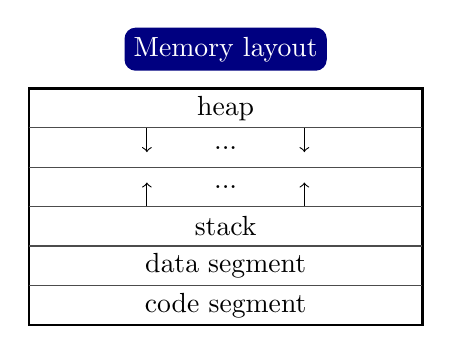
\begin{tikzpicture}
    \memorystack[size x=5cm,word size=1,nb blocks=6,addresses=0]
    \memorypush{code segment}
    \memorypush{data segment}
    \memorypush{stack}
    \memorypush{...}
    \memorypush{...}
    \memorypush{heap}
    \draw[->] (stack3-1.north) ++(-1cm,0) -- +(0,.3cm);
    \draw[->] (stack3-1.north) ++(1cm,0) -- +(0,.3cm);
    \draw[->] (stack6-1.south) ++(-1cm,0) -- +(0,-.3cm);
    \draw[->] (stack6-1.south) ++(1cm,0) -- +(0,-.3cm);
  \end{tikzpicture}
\end{frame}

\begin{frame}[fragile]
  \frametitle{The Stack}
  \begin{block}{Main characteristics}
    \begin{itemize}
    \item allocation on the stack stays in scope as long as it is on the stack \\
    It is destroyed when it is popped off the stack.
    \item memory allocated on the stack is known at compile time and can thus be accessed through a variable.
    \item the stack is relatively small, it is not a good idea to allocate large arrays, structures or classes
    \end{itemize}
  \end{block}
\end{frame}

\begin{frame}[fragile]
  \frametitle{Object allocation on the stack}
  \begin{block}{On the stack}
    \begin{itemize}
    \item object are created when declared (constructor called)
    \item object are destructed when out of scope (destructor is called)
    \end{itemize}
  \end{block}
  \begin{cppcode}
    {
      MyFirstClass a; // default constructor called
      ...
    }  // destructor called

    int f() {
      MyFirstClass a(3); // constructor called
      ...
    } // destructor called
  \end{cppcode}
\end{frame}

\begin{frame}[fragile]
  \frametitle{The Heap}
  \begin{block}{Main characteristics}
    \begin{itemize}
    \item Allocated memory stays allocated until it is specifically deallocated
      \begin{itemize}
      \item beware memory leaks
      \end{itemize}
    \item Dynamically allocated memory must be accessed through pointers
    \item large arrays, structures, or classes should be allocated here
    \end{itemize}
  \end{block}
\end{frame}

\begin{frame}[fragile]
  \frametitle{Object allocation on the heap}
  \begin{block}{On the heap}
    \begin{itemize}
    \item object are created by calling {\it new} (constructor is called)
    \item object are destructed by calling {\it delete} (destructor is called)
    \end{itemize}
  \end{block}
  \begin{cppcode}
    {
      // default constructor called
      MyFirstClass *a = new MyFirstClass;
      ...
      delete a; // destructor is called
    }

    int f() {
      // constructor called
      MyFirstClass *a = new MyFirstClass(3);
      ...
    } // memory leak !!!
  \end{cppcode}
\end{frame}

\begin{frame}[fragile]
  \frametitle{Array allocation on the heap}
  \begin{block}{Arrays on the heap}
    \begin{itemize}
    \item arrays of objects are created by calling {\it new[]} \\
      default constructor is called for each object of the array
    \item arrays of object are destructed by calling {\it delete[]} \\
      destructor is called for each object of the array
    \end{itemize}
  \end{block}
  \begin{cppcode}
    {
      // default constructor called 10 times
      MyFirstClass *a = new MyFirstClass[10];
      ...
      delete[] a; // destructor called 10 times
    }
  \end{cppcode}
\end{frame}


\subsection[Exceptions]{Exceptions (Deprecated)}

\begin{frame}[fragile]
  \frametitle{Exceptions \hfill \deprecated}
  \begin{block}{The concept}
    \begin{itemize}
    \item exceptional Event breaking linearity of the code
    \item will be handled in dedicated place
    \end{itemize}
  \end{block}
  \begin{block}{Pratically}
    \begin{itemize}
    \item you can throw any object with {\it throw}
    \item you handle them using {\it try ... catch} blocks
    \end{itemize}
  \end{block}
  \begin{cppcode}
    try {
      if (0 == name) {
        throw std::string("Expected non empty name");
      }
      printf("%s\n", name);
    } catch (std::string e) {
      printf("empty name found\n");      
    }
  \end{cppcode}
\end{frame}

\begin{frame}[fragile]
  \frametitle{Exceptions \hfill \deprecated}
  \begin{block}{Rules}
    \begin{itemize}
    \item exception will skip all code until next {\it catch}
    \begin{itemize}
      \item still destructors are called when exiting scopes
      \item but your own cleanup may not be
    \end{itemize}
    \item {\it catch} is selective on the exception type
    \end{itemize}
  \end{block}
  \begin{multicols}{2}
    \begin{cppcode*}{fontsize=\scriptsize,gobble=2}
      class ZeroDivide {};
      
      int divide(int a, int b) {
        if (0 == b) {
          throw ZeroDivide();
        }
        return a/b;
      }
    \end{cppcode*}
    \columnbreak
    \begin{cppcode*}{fontsize=\scriptsize,gobble=2,firstnumber=9} 
      int func(char* value) {
        try {
          errno = 0;
          long l = strtol(value,0,10);
          if (errno) {
            throw string("Bad Value");
          }
          divide(100, l);
        } catch (string e) {
          printf("%s\n", e.c_str());
        } catch (ZeroDivide e2) {
          printf("Division error\n");
        }
      }
    \end{cppcode*}
  \end{multicols}
\end{frame}

\begin{frame}[fragile]
  \frametitle{Controlling exceptions \hfill \deprecated}
  \begin{block}{Declaring expected exceptions}
    \begin{itemize}
    \item each function can declare a set of expected exceptions
    \item using the {\it throw} statement in its declaration
    \item other exceptions won't exit the scope of the function
      \begin{itemize}
      \item instead, the {\it unexpected} handler is called
      \item by default, it terminates the program
      \end{itemize}
    \end{itemize}
  \end{block}
  \pause
  \begin{cppcode}
    int func(int a) throw(int) {
      if (0 == a) {
        throw 2;  // ok, goes out
      } else {
        throw "hello"; // std::unexpected called
      }
    }
  \end{cppcode}
\end{frame}  

\begin{frame}[fragile]
  \frametitle{Controlling exceptions \hfill \deprecated}
  \begin{block}{Good to know}
    \begin{itemize}
    \item The check in done at runtime, not at compile time
      \begin{itemize}
      \item unlike Java
      \end{itemize}
    \item When the {\it throw} clause is absent, any exception can go out
    \item To block all exceptions, use {\it throw()}
    \end{itemize}
  \end{block}
  \pause
  \begin{cppcode}
    int func(int a) {
      // any exception can go out
    }
    int otherfunc(int a) throw() {
      // no exception can go out
    }
  \end{cppcode}
\end{frame}  

\section[More]{Core modern \cpp}

\subsection[const]{Constness}

\begin{frame}[fragile]
  \frametitlecpp[98]{Constness}
  \begin{block}{The {\it const} keyword}
    \begin{itemize}
    \item indicate that the element to the left is constant
    \item this element won't be modifiable in the future
    \item this is all checked at compile time
    \end{itemize}
  \end{block}
  \begin{cppcode}
    // standard syntax
    int const i = 6;

    // error : i is constant
    i = 5;

    // also ok, when nothing on the left,
    // const applies to the element on the right
    const int j = 6;
  \end{cppcode}
\end{frame}

\begin{frame}[fragile]
  \frametitlecpp[98]{Constness and pointers}
  \begin{cppcode}
    // pointer to a constant integer
    int a = 1, b = 2;
    int const *i = &a;
    *i = 5; // error, int is const
    i = &b; // ok, pointer is not const

    // constant pointer to an integer
    int * const j = &a;
    *j = 5; // ok, value can be changed
    j = &b; // error, pointer is const

    // constant pointer to a constant integer
    int const * const k = &a;
    *k = 5; // error, value is const
    k = &b; // error, pointer is const
  \end{cppcode}
\end{frame}

\begin{frame}[fragile]
  \frametitlecpp[98]{Method constness}
  \begin{block}{The {\it const} keyword for class functions}
    \begin{itemize}
    \item indicate that the function does not modify the object
    \item in other words, {\it this} is a pointer to constant object
    \end{itemize}
  \end{block}
  \begin{cppcode}
    struct Example {
      void foo() const  {
        m_member = 0; // Error : function is constant
      }
      int m_member;
    };
  \end{cppcode}
\end{frame}

\begin{frame}[fragile]
  \frametitlecpp[98]{Method constness}
  \begin{block}{Constness is part of the type}
    \begin{itemize}
    \item const T and T are different types
    \item however, T is automatically cast to const T when needed
    \end{itemize}
  \end{block}
  \begin{cppcode}
    void func(int & a);
    void funcConst(int const & a);

    int a = 0;
    int const b = 0;

    func(a);      // ok
    func(b);      // error
    funcConst(a); // ok
    funcConst(b); // ok
  \end{cppcode}
\end{frame}

\begin{frame}[fragile]
  \frametitlecpp[98]{constness}
  \begin{alertblock}{Exercise Time}
    \begin{itemize}
    \item go to code/constness
    \item open constplay.cpp
    \item try to find out which lines won't compile
    \item check your guesses by compiling for real
    \end{itemize}
  \end{alertblock}
\end{frame}

\subsection[cstexpr]{Constant Expressions}

\begin{frame}[fragile]
  \frametitlecpp[11]{Generalized Constant Expressions}
  \begin{block}{Reason of being}
    \begin{itemize}
    \item compute constant expressions at compile time
    \item even if non trivial
    \end{itemize}
  \end{block}
  \pause
  \begin{exampleblock}{Example}
    \begin{cppcode*}{}
      constexpr int f(int x) {
        return x > 1 ? x * f(x - 1) : 1;
      }
      constexpr int a = f(5); // computed at compile time
    \end{cppcode*}
  \end{exampleblock}
\end{frame}

\begin{frame}[fragile]
  \frametitlecpp[11]{Static Assertions}
  \begin{block}{static\_assert declaration}
    \begin{itemize}
    \item Performs compile time assertions; meaning a failed assertion stops compilation
    \item The expression has to be a constexpr boolean expression
    \item Purely evaluated at compile time, no effect at runtime
    \item Often used in template programming to make assertion on types, can be
      used to validate boolean compile time expressions
    \end{itemize}
  \end{block}
  \pause
  \begin{exampleblock}{Example}
    \begin{cppcode*}{}
      constexpr int f(int x) {
        return x > 1 ? x * f(x - 1) : 1;
      }
      static_assert(f(5)==120,"Expected f(5) to be 120!");
    \end{cppcode*}
  \end{exampleblock}
\end{frame}


\begin{frame}[fragile]
  \frametitlecpp[11]{Generalized Constant Expressions(2)}
   \begin{alertblock}{Few limitations in C++14 (more in C++11)}
    \begin{itemize}
    \item function's body cannot contain try-catch or static variables
    \item arguments should be constexpr or literals in order to benefit from compile time computation
    \end{itemize}
  \end{alertblock}
  \begin{block}{Notes}
    \begin{itemize}
    \item classes can have constexpr functions
    \item objects can be constexpr
      \begin{itemize}
      \item if the constructor of their class is
      \end{itemize}
    \item a constexpr function can also be used normally
    \item but a constexpr variable has to be evaluated at compile time
    \end{itemize}
  \end{block}
\end{frame}

\begin{frame}[fragile]
  \frametitlecpp[11]{Real life example}
  \begin{cppcode*}{}
    constexpr float toSI(const float v, const char unit) {
      switch (unit) {
      case 'k': return 1000*v;
      case 'm': return 0.001*v;
      case 'y': return 0.9144*v;
      case 'i': return 0.0254*v;
      ...
      default: return v;
      }
    }
    constexpr float fromSI(const float v, const char unit) {
      switch (unit) {
        case 'k': return 0.001*v;
        case 'y': return 1.093*v;
      ...
      }
    }
  \end{cppcode*}
\end{frame}

\begin{frame}[fragile]
  \frametitlecpp[11]{Real life example(2)}
  \begin{cppcode*}{}
    class DimLength {
      const float m_value;
    public:
      constexpr DimLength(const float v, const char unit):
        m_value(toSI(v, unit)) {
      }
      constexpr float get(const char unit) const {
        return fromSI(m_value, unit);
      }
    };
    constexpr DimLength km(1, 'k');
    constexpr float km_y = km.get('y');
    constexpr float km_i = km.get('i');
    static_assert(km_y == 1093, "expected km == 1093 yards!");
  \end{cppcode*}
\end{frame}

\subsection[except]{Exceptions}

\begin{frame}[fragile]
  \frametitlecpp[98]{Exceptions}
  \begin{block}{The concept}
    \begin{itemize}
    \item exceptional event breaking linearity of the code
    \item will be handled in dedicated place
    \end{itemize}
  \end{block}
  \begin{block}{Practically}
    \begin{itemize}
    \item you can throw any object with {\it throw}
    \item you handle them using {\it try ... catch} blocks
    \end{itemize}
  \end{block}
  \begin{cppcode}
    try {
      if (0 == name) {
        throw std::string("Expected non empty name");
      }
      printf("%s\n", name);
    } catch (std::string& e) {
      printf("empty name found\n");
    }
  \end{cppcode}
\end{frame}

\begin{frame}[fragile]
  \frametitlecpp[98]{Exceptions}
  \begin{block}{Rules}
    \begin{itemize}
    \item exception will skip all code until next {\it catch}
    \begin{itemize}
      \item still destructors are called when exiting scopes
      \item but your own cleanup may not be
    \end{itemize}
    \item {\it catch} is selective on the exception type
    \end{itemize}
  \end{block}
  \begin{multicols}{2}
    \begin{cppcode*}{fontsize=\scriptsize,gobble=2}
      struct ZeroDivide {};

      int divide(int a, int b) {
        if (0 == b) {
          throw ZeroDivide();
        }
        return a/b;
      }
    \end{cppcode*}
    \columnbreak
    \begin{cppcode*}{fontsize=\scriptsize,gobble=2,firstnumber=9}
      int func(char* value) {
        try {
          errno = 0;
          long l = strtol(value,0,10);
          if (errno) {
            throw string("Bad Value");
          }
          divide(100, l);
        } catch (string& e) {
          printf("%s\n", e.c_str());
        } catch (ZeroDivide e2) {
          printf("Division error\n");
        }
      }
    \end{cppcode*}
  \end{multicols}
\end{frame}

\begin{frame}[fragile]
  \frametitlecpp[98]{Controlling exceptions \hfill \deprecated}
  \begin{block}{Declaring expected exceptions}
    \begin{itemize}
    \item each function can declare a set of expected exceptions
    \item using the {\it throw} statement in its declaration
    \item other exceptions won't exit the scope of the function
      \begin{itemize}
      \item instead, the {\it unexpected} handler is called
      \item by default, it terminates the program
      \end{itemize}
    \end{itemize}
  \end{block}
  \pause
  \begin{cppcode}
    int func(int a) throw(int) {
      if (0 == a) {
        throw 2;  // ok, goes out
      } else {
        throw "hello"; // std::unexpected called
      }
    }
  \end{cppcode}
\end{frame}

\begin{frame}[fragile]
  \frametitlecpp[98]{Controlling exceptions \hfill \deprecated}
  \begin{block}{Good to know}
    \begin{itemize}
    \item The check is done at runtime, not at compile time
      \begin{itemize}
      \item unlike Java
      \end{itemize}
    \item When the {\it throw} clause is absent, any exception can go out
    \item To block all exceptions, use {\it throw()}
    \end{itemize}
  \end{block}
  \pause
  \begin{cppcode}
    int func(int a) {
      // any exception can go out
    }
    int otherfunc(int a) throw() {
      // no exception can go out
    }
  \end{cppcode}
\end{frame}

\begin{frame}[fragile]
  \frametitlecpp[11]{Deprecation of \cpp98 exceptions}
  \begin{block}{}
    After a lot of thinking and experiencing, the conclusions of the community on exception handling are :
    \begin{itemize}
    \item Never write an exception specification
    \item Except possibly an empty one
    \end{itemize}
  \end{block}
  \pause
  \begin{alertblock}{Some of the reasons}
    \begin{itemize}
    \item throw specification is runtime only
      \begin{itemize}
      \item does not allow compiler optimizations
      \item on the contrary forces extra checks
      \item generally terminates your program if violated
      \end{itemize}
    \item throw specification clashes with templates
      \begin{itemize}
      \item one cannot ``template'' the throw clause
      \end{itemize}
    \end{itemize}
  \end{alertblock}
\end{frame}

\begin{frame}[fragile]
  \frametitlecpp[11]{What remains}
  \begin{block}{throw is dead}
    \begin{itemize}
    \item throw statements are deprecated
    \item even throw() (no exceptions)
    \end{itemize}
  \end{block}
  \pause
  \begin{exampleblock}{long live noexcept}
    \begin{itemize}
    \item noexcept a somehow equivalent to throw()
    \item but is checked at compile time
    \item so allows compiler optimizations
    \end{itemize}
  \end{exampleblock}
\end{frame}

\begin{frame}[fragile]
  \frametitlecpp[11]{Full power of noexcept}
  \begin{block}{3 uses of noexcept}
    \begin{itemize}
    \item standalone
      \begin{cppcode*}{gobble=2, linenos=false}
        int f() noexcept;
      \end{cppcode*}
    \item as an expression saying whether exceptions can be sent
      \begin{cppcode*}{gobble=2, linenos=false}
        int f() noexcept(sizeof(long) == 8);
      \end{cppcode*}
    \item as an operator to know whether a function launches exceptions
      \begin{cppcode*}{gobble=2, linenos=false}
        template <typename T> void foo()
             noexcept(noexcept(T())) {}
      \end{cppcode*}
   \end{itemize}
  \end{block}
\end{frame}

\subsection[mv]{Move semantics}

\begin{frame}[fragile]
  \frametitlecpp[11]{Move semantics : the problem}
  \begin{exampleblock}{Non efficient code}
    \begin{cppcode*}{}
      void swap(std::vector<int> &a,
                std::vector<int> &b) {
        std::vector<int> c = a;
        a = b;
        b = c;
      }
      std::vector<int> v(10000), w(10000);
      for (int i = 0; i < 10000; i++) v[i] = i;
      for (int i = 0; i < 10000; i++) w[i] = i*i;
      swap(v, w);
    \end{cppcode*}
  \end{exampleblock}
  \pause
  \begin{alertblock}{What really happens during swap}
    \begin{itemize}
    \item 10k allocations + 10k releases
    \item 30k copies
    \end{itemize}
  \end{alertblock}
\end{frame}

\begin{frame}[fragile]
  \frametitlecpp[11]{Move semantics : the problem}
  \begin{exampleblock}{Dedicated efficient code}
    \begin{cppcode*}{}
      std::vector<int> v(10000), w(10000);
      for (int i = 0; i < 10000; i++) v[i] = i;
      for (int i = 0; i < 10000; i++) w[i] = i*i;
      v.swap(w);
      \end{cppcode*}
  \end{exampleblock}
  \pause
  \begin{block}{What probably happens during swap}
    \begin{itemize}
    \item 1 allocations + 1 releases
    \item 3 copies
    \end{itemize}
    only the pointers to underlying arrays were swapped
  \end{block}
\end{frame}

\begin{frame}[fragile]
  \frametitlecpp[11]{Move semantics : the problem}
  \begin{exampleblock}{Another non efficient code}
    \begin{cppcode*}{}
      std::vector<int> vrandom(unsigned int n) {
        std::vector<int> result(n);
        for (int i = 0; i < n; i++) {
          result[i] = rand();
        }
        return result;
      }
      std::vector<int> v = vrandom(10000);
    \end{cppcode*}
  \end{exampleblock}
  \pause
  \begin{alertblock}{What really happens during assignment}
    \begin{itemize}
    \item 10k allocations + 10k releases
    \item 10k copies
    \end{itemize}
    Note that in this case, the compiler may optimize the copy away.
  \end{alertblock}
\end{frame}

\begin{frame}[fragile]
  \frametitlecpp[11]{Move semantics : the problem}
  \begin{exampleblock}{Dedicated efficient way}
    \begin{cppcode*}{}
      void vrandom(unsigned int n, std::vector<int> &v) {
        v.resize(n);
        for (int i = 0; i < n; i++) {
          v[i] = rand();
        }
      }
      std::vector<int> v;
      vrandom(10000, v);
    \end{cppcode*}
  \end{exampleblock}
  \pause
  \begin{block}{The ideal situation}
    Have a way to express that we move the vector's content
  \end{block}
\end{frame}

\begin{frame}[fragile]
  \frametitlecpp[11]{Move semantics}
  \begin{block}{The idea}
    \begin{itemize}
      \item a new type of reference : rvalue references
      \begin{itemize}
      \item used for move semantic
      \item denoted by \&\&
      \end{itemize}
      \item 2 new members in every class, with move semantic :
      \begin{description}
      \item[a move constructor] similar to copy constructor
      \item[a move assignment operator] similar to assignment operator (now called copy assignment operator)
      \end{description}
    \end{itemize}
  \end{block}
  \pause
  \begin{exampleblock}{Practically}
    \begin{cppcode*}{}
      T(T const &  other); // copy construction
      T(      T&& other); // move construction
      T& operator=(T const &  other); // copy assignment
      T& operator=(      T&& other); // move assignment
    \end{cppcode*}
  \end{exampleblock}
\end{frame}

\begin{frame}[fragile]
  \frametitlecpp[11]{Move semantics}
  \begin{block}{A few important points concerning move semantic}
    \begin{itemize}
    \item the whole STL understands move semantics
    \item move assignment operator is allowed to destroy source
      \begin{itemize}
      \item so do not reuse source afterward
      \item still, I advice to never leave inconsistent objects
      \end{itemize}
    \item if not implemented, move falls back to copy version
    \item move is called by the compiler whenever possible
      \begin{itemize}
      \item e.g. when passing temporary
      \end{itemize}
    \end{itemize}
  \end{block}
  \pause
  \begin{exampleblock}{Practically}
    \begin{cppcode*}{}
      T a;
      T b = a;      // 1. Copy assign
      T c = T(2);   // 2. Move assign
      T d = func(); // 3. Move assign
    \end{cppcode*}
  \end{exampleblock}
\end{frame}

\begin{frame}[fragile]
  \frametitlecpp[11]{Move semantics}
  \begin{block}{In some cases, you want to force a move}
    \begin{cppcode*}{}
      void swap(T &a, T &b) {
        T c = a;  // copy
        a = b;    // copy
        b = c;    // copy
      }
    \end{cppcode*}
  \end{block}
  \pause
  \begin{block}{There are mainly two ways}
    \begin{itemize}
    \item casting to an rvalue reference
    \item using the std::move function
    \end{itemize}
    \begin{cppcode*}{firstnumber=6}
      T a;
      T b = a;                   // Copy assign
      T c = static_cast<T&&>(a); // Move assign
      T d = std::move(a);        // Move assign
    \end{cppcode*}
  \end{block}
\end{frame}

\begin{frame}[fragile]
  \frametitlecpp[11]{Move semantics : the easy way}
  \begin{block}{Use copy and swap idiom}
    \begin{itemize}
    \item implement an efficient swap method for your class
      \begin{itemize}
      \item preferably outside the class so that it is symmetric
      \end{itemize}
    \item use swap for move constructor
      \begin{itemize}
      \item create empty object with constructor delegation
      \item swap it with source
      \end{itemize}
    \item use swap in move assignment
      \begin{itemize}
      \item pass parameter by value
      \item this should force creation of a local replica of source
      \item as we are in the move assignment \\
        our move constructor will be called \\
        and source will be filled with an empty object
      \item swap local object with *this
      \item let local object be destructed when exiting the method \\
        this will actually destroy the original content of the target
      \end{itemize}
    \end{itemize}
  \end{block}
\end{frame}

\begin{frame}[fragile]
  \frametitlecpp[11]{Move semantics : the easy way}
  \begin{exampleblock}{Practically}
    \begin{cppcode*}{}
      class Movable {
        Movable();
        Movable(Movable &&other) :
          Movable() {         // constructor delegation
          swap(*this, other);
        }
        Movable& operator=(Movable other) { // by value
          swap(*this, other);
          return *this;
        }
        friend void swap(Movable &a, Movable &b);
      };
      void swap(Movable &a, Movable &b);
    \end{cppcode*}
  \end{exampleblock}
\end{frame}

\begin{frame}[fragile]
  \frametitlecpp[11]{Move Semantic}
  \begin{alertblock}{Exercise Time}
    \begin{itemize}
    \item go to code/move
    \item look at the code and run it with callgrind
    \item understand how inefficient it is
    \item implement move semantic the easy way in NVector
    \item run with callgrind and see no improvement
    \item understand why and fix test.cpp
    \item see efficiency improvements
    \end{itemize}
  \end{alertblock}
  prerequisite : be able to use simple templated code
\end{frame}

\subsection[copy]{Copy elision}

\begin{frame}[fragile]
  \frametitlecpp[17]{Guaranteed copy elision}
  \begin{block}{What is copy elision}
    \begin{cppcode*}{}
      struct Foo { ... };
      Foo f() {
        return Foo();
      }
      int main() {
        // compiler was authorised to elide the copy
        Foo foo = f();
      }
    \end{cppcode*}
  \end{block}
  \begin{exampleblock}{From \cpp17 on}
    The elision is guaranteed.
  \end{exampleblock}
\end{frame}

\begin{frame}[fragile]
  \frametitlecpp[17]{Guaranteed copy elision}
  Allows to write code not allowed with \cpp14 (would not compile)
  \begin{block}{One case where the guarantee is needed}
    \begin{cppcode*}{}
      struct Foo {
        Foo() { ... }
        Foo(const Foo &) = delete;
        Foo(Foo &&) = delete;
      };
      Foo f() {
        return Foo();
      }
      int main() {
        Foo foo = f();
      }
    \end{cppcode*}
  \end{block}
\end{frame}

\subsection[\textless{}T\textgreater]{Templates}

\begin{frame}[fragile]
  \frametitlecpp[98]{Templates}
  \begin{block}{Concept}
    \begin{itemize}
    \item The \cpp way to write reusable code
      \begin{itemize}
        \item aka macros on steroids
      \end{itemize}
    \item Applicable to functions and objects
    \end{itemize}
  \end{block}
  \begin{cppcode}
    template<typename T>
    const T & max(const T &A, const T &B) {
      return A > B ? A : B;
    }

    template<typename T>
    struct Vector {
      int m_len;
      T* m_data;
    };
 \end{cppcode}
\end{frame}

\begin{frame}[fragile]
  \frametitlecpp[98]{Templates}
  \begin{alertblock}{Warning}
    These are really like macros
    \begin{itemize}
      \item they are compiled n times
      \item they need to be defined before used
      \begin{itemize}
        \item so all templated code has to be in headers
      \end{itemize}
      \item this may lead to longer compilation times and bigger libraries
    \end{itemize}
  \end{alertblock}
  \newsavebox{\codepiece}
  \begin{lrbox}{\codepiece}
    \begin{minipage}{.35\linewidth}
      \small
      \begin{cppcode*}{gobble=4}
        template<typename T>
        T func(T a) {
          return a;
        }
      \end{cppcode*}
    \end{minipage}
  \end{lrbox}
  \newsavebox{\codepiecea}
  \begin{lrbox}{\codepiecea}
    \begin{minipage}{.4\linewidth}
      \small
      \begin{cppcode*}{gobble=4,linenos=false}
        int func(int a) {
          return a;
        }
      \end{cppcode*}
    \end{minipage}
  \end{lrbox}
  \newsavebox{\codepieceb}
  \begin{lrbox}{\codepieceb}
    \begin{minipage}{.4\linewidth}
      \small
      \begin{cppcode*}{gobble=4,linenos=false}
        double func(double a) {
          return a;
        }
      \end{cppcode*}
    \end{minipage}
  \end{lrbox}
  \begin{tikzpicture}[rectangle,rounded corners]
    \draw node (template) [draw] {\usebox{\codepiece}}
          node (templatea) [draw] at (6cm,+1cm) {\usebox{\codepiecea}}
          node (templateb) [draw] at (6cm,-1cm) {\usebox{\codepieceb}};
    \draw[->,thick] (template) -- (templatea) node [above,midway,sloped] {\small func(3)};
    \draw[->,thick] (template) -- (templateb) node [below,midway,sloped] {\small func(5.2)};
  \end{tikzpicture}
\end{frame}

\begin{frame}[fragile]
  \frametitlecpp[98]{Templates}
  \begin{block}{Arguments}
    \begin{itemize}
    \item can be a class,
    \item you can have several
    \item last ones can have a default value
    \end{itemize}
  \end{block}
  \begin{cppcode*}{}
    template<typename KeyType=int, typename ValueType=KeyType>
    struct Map {
      void set(const KeyType &key, ValueType value);
      ValueType get(const KeyType &key);
    }

    Map<std::string, int> m1;
    Map<float> m2;   // Map<float, float>
    Map<> m3;        // Map<int, int>
  \end{cppcode*}
\end{frame}

\begin{frame}[fragile]
  \frametitlecpp[98]{Templates implementation}
  \begin{cppcode*}{}
    template<typename KeyType=int, typename ValueType=KeyType>
    struct Map {
      void set(const KeyType &key, ValueType value);
      ValueType get(const KeyType &key);
    }

    template<typename KeyType, typename ValueType>
    void Map<KeyType, ValueType>::set
       (const KeyType &key, ValueType value) {
      ...
    }

    template<typename KeyType, typename ValueType>
    ValueType Map<KeyType, ValueType>::get
       (const KeyType &key) {
      ...
    }
  \end{cppcode*}
\end{frame}

\begin{frame}[fragile]
  \frametitle{Non-type template parameter \hfill \cpp98 / \cpp17 / \cpp20}
  \begin{block}{template parameters can also be a value}
    \begin{itemize}
    \item integral types, pointer, enums in \cpp98
    \item auto in \cpp17
    \item floats and literals in \cpp20
    \end{itemize}
  \end{block}
  \begin{cppcode*}{}
    template<unsigned int N> struct Polygon {
      Polygon(float radius);
      float perimeter() {return 2*N*sin(PI/N)*m_radius;}
      float m_radius;
    };
  \end{cppcode*}
\end{frame}

\begin{frame}[fragile]
  \frametitlecpp[98]{Templates}
  \begin{block}{Specialization}
    templates can be specialized for given values of their parameter
  \end{block}
  \begin{cppcode*}{}
    template<typename F, unsigned int N> struct Polygon {
      Polygon(F radius) : m_radius(radius) {}
      F perimeter() {return 2*N*sin(PI/N)*m_radius;}
      F m_radius;
    };

    template<typename F>
    struct Polygon<F, 6> {
      Polygon(F radius) : m_radius(radius) {}
      F perimeter() {return 6*m_radius;}
      F m_radius;
    };
  \end{cppcode*}
\end{frame}

\begin{frame}[fragile]
  \frametitlecpp[98]{The full power of templates}
  \begin{alertblock}{Exercise Time}
    \begin{itemize}
    \item go to code/templates
    \item look at the OrderedVector code
    \item compile and run playwithsort.cpp. See the ordering
    \item modify playwithsort.cpp and reuse OrderedVector with Complex
    \item improve OrderedVector to template the ordering
    \item test reverse ordering of strings (from the last letter)
    \item test order based on {\color{blue} \href{https://en.wikipedia.org/wiki/Taxicab_geometry}{Manhattan distance}} with complex type
    \item check the implementation of Complex
    \item try ordering complex of complex
    \end{itemize}
  \end{alertblock}
\end{frame}

\subsection[STL]{The STL}

\begin{frame}[fragile]
  \frametitlecpp[98]{The Standard Template Library}
  \begin{block}{What it is}
    \begin{itemize}
    \item A library of standard templates
    \item Everything you need, or ever dreamed of
      \begin{itemize}
      \item strings, containers, iterators
      \item algorithms, functions, sorters
      \item functors, allocators
      \item ...
      \end{itemize}
    \item Portable
    \item Reusable
    \item Efficient
    \end{itemize}
  \end{block}
  \pause
  \begin{alertblock}{Just use it}
    and adapt it to your needs, thanks to templates
  \end{alertblock}
\end{frame}

\begin{frame}[fragile,label=STLcode]
  \frametitlecpp[11]{STL in practice}
  \begin{cppcode*}{}
    #include <vector>
    #include <algorithm>

    std::vector<int> vi{5, 3, 4}; // initializer list
    std::vector<int> vr(3); // constructor taking int

    std::transform(vi.begin(), vi.end(),      // range1
                   vi.begin(),          // start range2
                   vr.begin(),          // start result
                   std::multiplies<int>()); // function

    for(auto n : vr) {
      std::cout << n << ' ';
    }
  \end{cppcode*}
\end{frame}

\begin{frame}[fragile]
  \frametitlecpp[98]{STL's concepts}
  \begin{block}{containers}
    \begin{itemize}
    \item a structure containing data
    \item with a given way of handling it
    \item irrespective of
      \begin{itemize}
      \item the data itself (templated)
      \item the memory allocation of the structure (templated)
      \item the algorithms that may use the structure
      \end{itemize}
    \item examples
      \begin{itemize}
      \item string
      \item tuple, list, vector, deque
      \item map, set, multimap, multiset, hash\_map, hash-set, ...
      \item stack, queue, priority\_queue
      \end{itemize}
    \end{itemize}
  \end{block}
\end{frame}

\begin{frame}[fragile]
  \frametitlecpp[98]{STL's concepts}
  \begin{block}{iterators}
    \begin{itemize}
    \item generalization of pointers
    \item allowing iteration over some data
    \item irrespective of
      \begin{itemize}
      \item the container used (templated)
      \item the data itself (container is templated)
      \item the consumer of the data (templated algorithm)
      \end{itemize}
    \item examples
      \begin{itemize}
      \item iterator
      \item reverse\_iterator
      \item const\_iterator
      \end{itemize}
    \end{itemize}
  \end{block}
\end{frame}

\begin{frame}[fragile]
  \frametitlecpp[98]{STL's concepts}
  \begin{block}{algorithms}
    \begin{itemize}
    \item implementation of an algorithm working on data
    \item with a well defined behavior (defined complexity)
    \item irrespective of
      \begin{itemize}
      \item the data handled
      \item the container where data live
      \item the iterator used to go through data
      \end{itemize}
    \item examples
      \begin{itemize}
      \item for\_each, find, find\_if, count, count\_if, search
      \item copy, swap, transform, replace, fill, generate
      \item remove, remove\_if
      \item unique, reverse, rotate, random, partition
      \item sort, partial\_sort, merge, min, max
      \item lexicographical\_compare, iota, accumulate, partial\_sum
      \end{itemize}
    \end{itemize}
  \end{block}
\end{frame}

\begin{frame}[fragile]
  \frametitlecpp[98]{STL's concepts}
  \begin{block}{functions / functors}
    \begin{itemize}
      \item generic utility functions/functors
      \item mostly useful to be passed to STL algorithms
    \item implemented independently of
      \begin{itemize}
      \item the data handled (templated)
      \item the context (algorithm) calling it
      \end{itemize}
    \item examples
      \begin{itemize}
      \item plus, minus, multiply, divide, modulus, negate
      \item equal\_to, less, greater, less\_equal, ...
      \item logical\_and, logical\_or, logical\_not
      \item identity, project1st, project2nd
      \item binder1st, binder2nd, unary\_compose, binary\_compose
      \end{itemize}
    \end{itemize}
  \end{block}
\end{frame}

\againframe{STLcode}

\begin{frame}[fragile]
  \frametitlecpp[98]{STL in practice using \cpp98}
  \begin{cppcode*}{}
    #include <vector>
    #include <algorithm>

    std::vector<int> vi, vr(3);
    vi.push_back(5); vi.push_back(3); vi.push_back(4);

    std::transform(vi.begin(), vi.end(),      // range1
                   vi.begin(),          // start range2
                   vr.begin(),          // start result
                   std::multiplies<int>()); // function

    for(std::vector<int>::iterator it = vr.begin();
        it != vr.end();
        it++) {
      std::cout << *it << ' ';
    };
  \end{cppcode*}
\end{frame}

\begin{frame}[fragile]
  \frametitlecpp[98]{STL and functors}
  \begin{cppcode}
    // Finds the first element in a list that lies in
    // the range from 1 to 10.
    list<int> L;
    ...
    list<int>::iterator in_range =
      find_if(L.begin(), L.end(),
              compose2(logical_and<bool>(),
                       bind2nd(greater_equal<int>(), 1),
                       bind2nd(less_equal<int>(), 10)));

    // Computes sin(x)/(x + DBL_MIN) for elements of a range.
    transform(first, last, first,
              compose2(divides<double>(),
                       ptr_fun(sin),
                       bind2nd(plus<double>(), DBL_MIN)));
  \end{cppcode}
\end{frame}

\begin{frame}[fragile]
  \frametitlecpp[98]{Welcome to lego programming !}
  \begin{block}{}
    \pgfdeclareimage[height=0.5cm]{AtlasLego}{AtlasLego.jpg}
    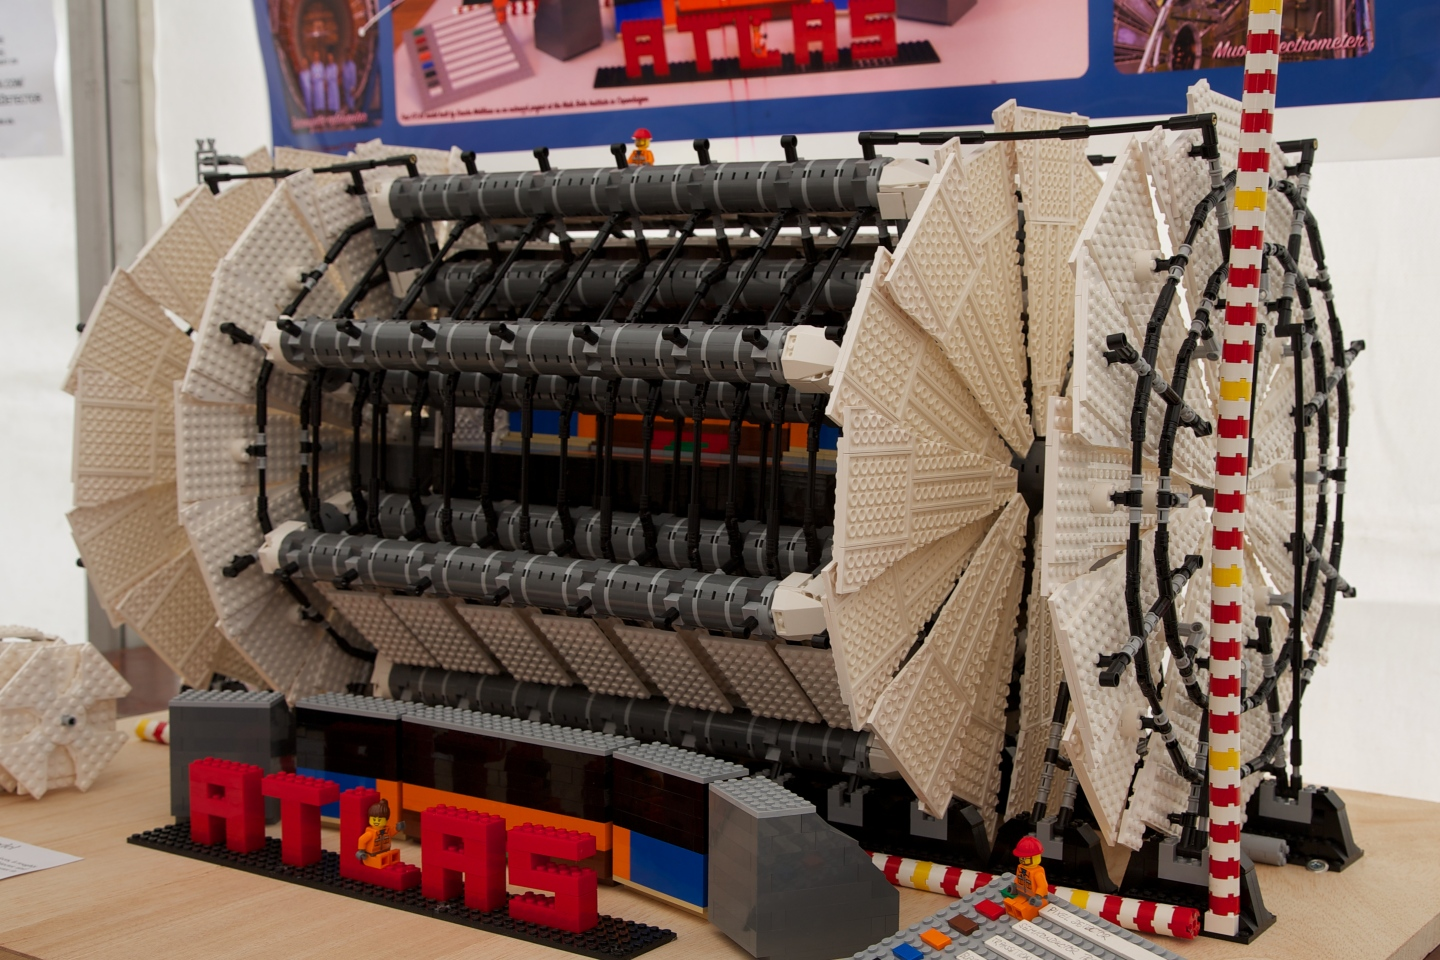
\includegraphics[width=\linewidth]{AtlasLego}
  \end{block}
\end{frame}

\begin{frame}[fragile]
  \frametitlecpp[98]{Using the STL}
  \begin{alertblock}{Exercise Time}
    \begin{itemize}
    \item go to code/stl
    \item look at the non STL code in randomize.nostl.cpp
      \begin{itemize}
        \item it creates a vector of ints at regular intervals
        \item it randomizes them
        \item it computes differences between consecutive ints
        \item and the mean and variance of it
      \end{itemize}
    \item open randomize.cpp and complete the ``translation'' to STL
    \item see how easy it is to reuse the code with complex numbers
    \end{itemize}
  \end{alertblock}
\end{frame}

\begin{frame}[fragile]
  \frametitlecpp[98]{Using the STL}
  \begin{alertblock}{Some last warning}
    You may find the STL quite difficult to use.
    \begin{itemize}
    \item template syntax is simply awful
    \item it is hard to debug (compilers spit out mostly garbage)
    \end{itemize}
    However, this has improved a lot with \cpp11 \\
    And will again in \cpp20 with concepts
  \end{alertblock}
\end{frame}

\begin{frame}[fragile]
  \frametitlecpp[11]{Loops and auto keyword with the STL}
  \begin{block}{Old way}
    \begin{cppcode*}{}
      std::vector<int> a = ...;
      int sum = 0;
      for (std::vector<int>::iterator it = v.begin();
           it != v.end(); it++) {
        sum += *it;
      }
    \end{cppcode*}
  \end{block}
  \pause
  \begin{block}{New way}
    \begin{cppcode*}{firstnumber=7}
      std::vector<int> v = ...;
      int sum = 0;
      for (auto a : v) { sum += a; }
    \end{cppcode*}
  \end{block}
  \pause
  \begin{exampleblock}{STL way}
    \begin{cppcode*}{firstnumber=10}
      std::vector<int> v = ...;
      int sum = std::accumulate(v.begin(), v.end(), 0);
    \end{cppcode*}
  \end{exampleblock}
\end{frame}

\subsection{More STL}

\begin{frame}[fragile]
  \frametitlecpp[17]{Some new STL types}
  \begin{block}{\texttt{std::optional}}
    \begin{itemize}
    \item manages an optional contained value
    \item contextually converted to bool
    \item useful for the return value of a function that may fail
    \end{itemize}
  \end{block}
  \begin{block}{\texttt{std::any}}
    \begin{itemize}
    \item a type-safe container for single values of any type
    \item the \texttt{any\_cast} function provides type-safe access
    \item and throws \texttt{std::bad\_any\_cast} for bad access
    \end{itemize}
  \end{block}
  \begin{block}{\texttt{std::variant}}
    \begin{itemize}
    \item a type-safe union
    \item \texttt{std::get} reads the value of the variant
    \item and throws \texttt{std::bad\_variant\_access} for bad accesses
    \end{itemize}
  \end{block}
\end{frame}

\begin{frame}[fragile]
  \frametitlecpp[11]{non-member begin and end}
  \begin{alertblock}{The problem in \cpp98}
    STL containers and arrays have different syntax for loop
    \vspace{-1mm}
    \begin{cppcode*}{}
      std::vector<int> v;
      int a[] = {1,2,3};
      for(auto it = v.begin(); it != v.end(); it++) {...}
      for(int i = 0; i < 3; i++) {...}
    \end{cppcode*}
  \end{alertblock}
  \pause
  \begin{block}{A new syntax}
    \begin{cppcode*}{firstnumber=5}
      for(auto it = begin(v); it != end(v); it++) {...}
      for(auto i = begin(a); i != end(a); i++) {...}
    \end{cppcode*}
  \end{block}
  \pause
  \begin{exampleblock}{Allowing the best syntax}
    \begin{cppcode*}{firstnumber=7}
      for(auto & element : v) {...}
      for(auto & element : a) {...}
    \end{cppcode*}
  \end{exampleblock}
\end{frame}

\begin{frame}[fragile]
  \frametitlecpp[17]{Structured Binding Declarations}
  Helps when using tuples as a return type.\\
  Automatically creates variables and ties them.
  \begin{alertblock}{\cpp14}
    \begin{cppcode*}{}
      void foo(std::tuple<int, double, long> tuple) {
        int a = 0;
        double b = 0.0;
        long c = 0;
        // a, b, c need to be declared first
        std::tie(a, b, c) = tuple;
    \end{cppcode*}
  \end{alertblock}
  \begin{exampleblock}{\cpp17}
    \begin{cppcode*}{firstnumber=7}
      void foo(std::tuple<int, double, long> tuple) {
      auto [ a, b, c ] = tuple;
    \end{cppcode*}
  \end{exampleblock}
\end{frame}

\subsection[$\lambda$]{Lambdas}

\begin{frame}[fragile]
  \frametitlecpp[11]{Function return type}
  \begin{block}{A new way to specify function's return type}
    \begin{cppcode*}{linenos=false}
      ReturnType fn_name(ArgType1, ArgType2);  //old
      auto fn_name(ArgType1, ArgType2) -> ReturnType;
    \end{cppcode*}
  \end{block}
  \pause
  \begin{block}{Advantages}
    \begin{itemize}
    \item Allows to simplify inner type definition
      \begin{cppcode*}{gobble=4}
        class TheClass {
          using inner_type = int;
          inner_type func();
        }
        TheClass::inner_type TheClass::func() {...}
        auto TheClass::func() -> inner_type {...}
      \end{cppcode*}
    \item C++14: ReturnType is not mandatory, compiler can deduce it
    \item will be used for lambdas
    \end{itemize}
  \end{block}
\end{frame}


\begin{frame}[fragile]
  \frametitlecpp[11]{Lambdas}
  \begin{block}{Definition}
    a lambda is a function with no name
  \end{block}
  \pause
  \begin{exampleblock}{Python example}
    \begin{pythoncode*}{}
      data = [1,9,3,8,3,7,4,6,5]

      # without lambdas
      def isOdd(n):
        return n%2 == 1
      print(filter(isOdd, data))

      # with lambdas
      print(filter(lambda n:n%2==1, data))
    \end{pythoncode*}
  \end{exampleblock}
\end{frame}

\begin{frame}[fragile]
  \frametitlecpp[11]{\cpp Lambdas}
  \begin{block}{Simplified syntax}
    \begin{cppcode*}{gobble=2}
      [] (args) -> type {
        code;
      }
    \end{cppcode*}
    The type specification is optional
  \end{block}
  \begin{exampleblock}{Usage example}
    \begin{cppcode*}{firstnumber=4,gobble=2}
      std::vector<int> data{1,2,3,4,5};
      for_each(begin(data), end(data),
               [](int i) {
                 std::cout << "The square of " << i
                           << " is " << i*i << std::endl;
               });
    \end{cppcode*}
  \end{exampleblock}
\end{frame}


\begin{frame}[fragile]
  \frametitlecpp[11]{Capture}
  \begin{block}{Python code}
    \begin{pythoncode*}{}
      increment = 3
      data = [1,9,3,8,3,7,4,6,5]
      map(lambda x : x + increment, data)
    \end{pythoncode*}
  \end{block}
  \pause
  \begin{block}{First attempt in \cpp}
    \begin{cppcode*}{firstnumber=4}
      int increment = 3;
      std::vector<int> data{1,9,3,8,3,7,4,6,5};
      transform(begin(data), end(data), begin(data),
                [](int x) { return x+increment; });
    \end{cppcode*}
  \end{block}
  \pause
  \begin{alertblock}{Error}
    \begin{minted}[gobble=6]{text}
        error: 'increment' is not captured
          [](int x) { return x+increment; });
                                     ^
    \end{minted}
  \end{alertblock}
\end{frame}

\begin{frame}[fragile]
  \frametitlecpp[11]{Capture}
  \begin{block}{Variable capture}
    \begin{itemize}
    \item external variables need to be explicitly captured
    \item captured variables are listed within initial []
    \end{itemize}
  \end{block}
  \pause
  \begin{exampleblock}{Example}
    \begin{cppcode*}{}
      int increment = 3;
      std::vector<int> data{1,9,3,8,3,7,4,6,5};
      transform(begin(data), end(data), begin(data),
                [increment](int x) {
                  return x+increment;
                });
    \end{cppcode*}
  \end{exampleblock}
\end{frame}

\begin{frame}[fragile]
  \frametitlecpp[11]{Default capture is by value}
  \begin{exampleblock}{Code example}
    \begin{cppcode}
      int sum = 0;
      std::vector<int> data{1,9,3,8,3,7,4,6,5};
      for_each(begin(data), end(data),
              [sum](int x) { sum += x; });
    \end{cppcode}
  \end{exampleblock}
  \pause
  \begin{alertblock}{Error}
    \begin{minted}[gobble=4]{text}
      error: assignment of read-only variable 'sum'
               [sum](int x) { sum += x; });
    \end{minted}
  \end{alertblock}
  \pause
  \begin{block}{Explanation}
    By default, variables are captured by value
  \end{block}
\end{frame}

\begin{frame}[fragile]
  \frametitlecpp[11]{Capture by reference}
  \begin{exampleblock}{Simple example}
    In order to capture by reference, add '\&' before the variable
    \begin{cppcode*}{}
      int sum = 0;
      std::vector<int> data{1,9,3,8,3,7,4,6,5};
      for_each(begin(data), end(data),
              [&sum](int x) { sum += x; });
    \end{cppcode*}
  \end{exampleblock}
  \pause
  \begin{exampleblock}{Mixed case}
    One can of course mix values and references
    \begin{cppcode*}{firstnumber=5}
      int sum = 0, offset = 1;
      std::vector<int> data{1,9,3,8,3,7,4,6,5};
      for_each(begin(data), end(data),
              [&sum, offset](int x) {
                sum += x + offset;
              });
    \end{cppcode*}
  \end{exampleblock}
\end{frame}

\begin{frame}[fragile]
  \frametitlecpp[11]{Capture all}
  \begin{block}{by value}
    \begin{cppcode*}{linenos=false}
      [=](...) { ... };
    \end{cppcode*}
  \end{block}
  \pause
  \begin{block}{by reference}
    \begin{cppcode*}{linenos=false}
      [&](...) { ... };
    \end{cppcode*}
  \end{block}
  \pause
  \begin{block}{exceptions}
    \begin{cppcode*}{linenos=false}
      [&, b](...) { ... };
      [=, &b](...) { ... };
    \end{cppcode*}
  \end{block}
\end{frame}

\begin{frame}[fragile]
  \frametitlecpp[11]{Lambdas rather than functors}
  \begin{exampleblock}{Example}
    \begin{cppcode*}{}
      auto build_incrementer = [](int inc) {
        return [inc](int value) { return value + inc; };
      };
      auto inc1 = build_incrementer(1);
      auto inc10 = build_incrementer(10);
      int i = 0;
      i = inc1(i);   // i = 1
      i = inc10(i);  // i = 11
    \end{cppcode*}
  \end{exampleblock}
  \begin{block}{How it works}
    \begin{itemize}
      \item build\_incrementer returns a function object
      \item this function's behavior depends on a parameter
      \item note how {\it auto} is useful here !
    \end{itemize}
  \end{block}
\end{frame}

\begin{frame}[fragile]
  \frametitlecpp[11]{{\texttt lambda}s makes the STL usable}
  \begin{block}{Before lambdas}
    \begin{cppcode*}{}
      struct Incrementer {
        int m_inc;
        Incrementer(int inc) : m_inc(inc) {}
        int operator() (int value) {
          return value + m_inc;
        };
      };
      std::vector<int> v{1, 2, 3};
      std::transform(begin(v), end(v), begin(v),
                     Incrementer(1));
      for (auto a : v) std::cout << a << " ";
      \end{cppcode*}
    \end{block}
\end{frame}

\begin{frame}[fragile]
  \frametitlecpp[11]{{\texttt lambda}s makes the STL usable}
  \begin{exampleblock}{With lambdas}
    \begin{cppcode*}{}
      std::vector<int> v{1, 2, 3};
      std::transform(begin(v), end(v), begin(v),
                     [](int value) {
                       return value + 1;
                     });
      for (auto a : v) std::cout << a << " ";
    \end{cppcode*}
  \end{exampleblock}
  \pause
  \begin{alertblock}{Conclusion}
    Use the STL !
  \end{alertblock}
\end{frame}

\begin{frame}[fragile]
  \frametitlecpp[11]{Lambdas}
  \begin{alertblock}{Exercise Time}
    \begin{itemize}
    \item go to code/lambdas
    \item look at the code (it's the solution to the stl exercise)
    \item use lambdas to simplify it
    \end{itemize}
  \end{alertblock}
\end{frame}

\subsection[RAII]{pointers and RAII}

\begin{frame}[fragile]
  \frametitlecpp[98]{Pointers : why they are error prone ?}
  \begin{exampleblock}{They need initialization
      \hfill \onslide<2->{\textcolor{orange}{\bf Seg Fault}}}
    \begin{cppcode*}{xleftmargin=20pt}
      char *s;
      try {
        callThatThrows();
        s = (char*) malloc(...);
        strncpy(s, ...);
      } catch (...) { ... }
      bar(s);
    \end{cppcode*}
  \end{exampleblock}
  \pause
  \pause
  \vspace{-2cm}
  \begin{exampleblock}{They need to be released
      \hfill \onslide<4->{\textcolor{orange}{\bf Memory leak}}}
    \begin{cppcode*}{xleftmargin=20pt}
      char *s = (char*) malloc(...);
      strncpy(s, ...);
      if (0 != strncmp(s, ...)) return;
      foo(s);
      free(s);
    \end{cppcode*}
  \end{exampleblock}
  \pause
  \pause
  \vspace{-2cm}
  \begin{exampleblock}{They need clear ownership
      \hfill \onslide<6->{\textcolor{orange}{\bf Who should release ?}}}
    \begin{cppcode*}{xleftmargin=20pt}
      char *s = (char*) malloc(...);
      strncpy(s, ...);
      someVector.push_back(s);
      someSet.add(s);
      std::thread t1(vecConsumer, someVector);
      std::thread t2(setConsumer, someSet);
    \end{cppcode*}
  \end{exampleblock}
\end{frame}

\begin{frame}[fragile]
  \frametitlecpp[98]{This problem exists for any resource}
  \begin{exampleblock}{For example with a file}
    \begin{cppcode*}{}
      try {
        FILE *handle = std::fopen(path, "w+");
        if (0 == handle) { throw ... }
        if (std::fputs(str, handle) == EOF) {
          throw ...
        }
        fclose(handle);
      } catch (...) { ... }
    \end{cppcode*}
  \end{exampleblock}
\end{frame}

\begin{frame}
  \frametitlecpp[98]{Resource Acquisition Is Initialization (RAII)}
  \begin{block}{Practically}
    Use object semantic to acquire/release resources
    \begin{itemize}
    \item wrap the resource inside an object
    \item acquire resource via object constructor
    \item release resource in destructor
    \item create this object on the stack so that it is automatically destructed when leaving the scope, including in case of exception
    \end{itemize}
  \end{block}
\end{frame}

\begin{frame}[fragile]
  \frametitlecpp[98]{RAII in practice}
  \begin{exampleblock}{File class}
    \begin{cppcode*}{}
      class File {
      public:
        File(const char* filename) :
          m_file_handle(std::fopen(filename, "w+")) {
          if (m_file_handle == NULL) { throw ... }
        }
        ~File() { std::fclose(m_file_handle); }
        void write (const char* str) {
          if (std::fputs(str, m_file_handle) == EOF) {
            throw ...
          }
        }
      private:
        FILE* m_file_handle;
      };
    \end{cppcode*}
  \end{exampleblock}
\end{frame}

\begin{frame}[fragile]
  \frametitlecpp[98]{RAII usage}
  \begin{exampleblock}{Usage of File class}
    \begin{cppcode*}{}
      void log_function() {
        // file opening, aka resource acquisition
        File logfile("logfile.txt") ;

        // file usage
        logfile.write("hello logfile!") ;

        // file is automatically closed by the call to
        // its destructor, even in case of exception !
      }
    \end{cppcode*}
  \end{exampleblock}
\end{frame}

\begin{frame}[fragile]
  \frametitlecpp[11]{std::unique\_ptr}
  \begin{block}{an RAII pointer}
    \begin{itemize}
    \item wraps a regular pointer
    \item has move only semantic
      \begin{itemize}
      \item the pointer is only owned once
      \end{itemize}
    \item in \textless{}memory\textgreater{} header
    \end{itemize}
  \end{block}
  \pause
  \begin{exampleblock}{Usage}
    \begin{cppcode*}{}
      Foo *p = new Foo{};  // allocation
      std::unique_ptr<Foo> uptr(p);
      std::cout << uptr.get() << " points to "
                << uptr->someMember << std::endl;
      void f(std::unique_ptr<Foo> ptr);
      f(std::move(uptr)); // transfer of ownership
      // deallocation when exiting f
      std::cout << uptr.get() << std::endl; // 0
    \end{cppcode*}
  \end{exampleblock}
\end{frame}

\begin{frame}[fragile]
  \frametitlecpp[11]{Quiz}
  \begin{exampleblock}{}
    \begin{cppcode*}{}
      Foo *p = new Foo{};  // allocation
      std::unique_ptr<Foo> uptr(p);
      void f(std::unique_ptr<Foo> ptr);
      f(uptr); // transfer of ownership
    \end{cppcode*}
    What do you expect ?
  \end{exampleblock}
  \pause
  \begin{alertblock}{Compilation Error}
    \begin{minted}{text}
test.cpp:15:5: error: call to deleted constructor
of 'std::unique_ptr<Foo>'
  f(uptr);
    ^~~~
/usr/include/c++/4.9/bits/unique_ptr.h:356:7: note:
 'unique_ptr' has been explicitly marked deleted here
 unique_ptr(const unique_ptr&) = delete;
 ^
    \end{minted}
  \end{alertblock}
\end{frame}

\begin{frame}[fragile]
  \frametitlecpp[14]{std::make\_unique}
  \begin{block}{}
    \begin{itemize}
    \item allocates directly a unique\_ptr
    \item no new or delete calls anymore !
    \end{itemize}
  \end{block}
  \pause
  \begin{exampleblock}{make\_unique usage}
    \begin{cppcode*}{}
      // allocation of one Foo object,
      // calling constructor with one argument
      auto a = std::make_unique<Foo>(memberValue);
      std::cout << a.get() << " points to "
                << a->someMember << std::endl;
      // allocation of an array of Foos
      // calling default constructor
      auto b = std::make_unique<Foo[]>(10);
      // deallocations
    \end{cppcode*}
  \end{exampleblock}
\end{frame}

\begin{frame}[fragile]
  \frametitlecpp[11]{RAII or raw pointers}
  \begin{block}{When to use what ?}
    \begin{itemize}
    \item Always use RAII for allocations
    \item You thus never have to deallocate !
    \item Use raw pointers for observer functions (or references)
      \begin{itemize}
      \item remember that unique\_ptr is move only
      \end{itemize}
    \end{itemize}
  \end{block}
  \pause
  \begin{exampleblock}{A question of ownership}
    \begin{cppcode*}{}
      unique_ptr<T> producer();
      void observer(const T&);
      void modifier(T&);
      void consumer(unique_ptr<T>);
      unique_ptr<T> pt{producer()};
      observer(*pt);            // Keep ownership
      modifier(*pt);            // Keep ownership
      consumer(std::move(pt));  // Transfer ownership
    \end{cppcode*}
  \end{exampleblock}
\end{frame}

\begin{frame}[fragile]
  \frametitlecpp[11]{unique\_ptr usage summary}
  \begin{block}{It's about lifetime management}
    \begin{itemize}
    \item Use unique\_ptr in functions taking part to the lifetime management
    \item Otherwise use raw pointers or references
    \end{itemize}
  \end{block}
\end{frame}

\begin{frame}[fragile]
  \frametitlecpp[11]{shared\_ptr, make\_shared}
  \begin{block}{shared\_ptr : a reference counting pointer}
    \begin{itemize}
    \item wraps a regular pointer like unique\_ptr
    \item has move and copy semantic
    \item uses internally reference counting
      \begin{itemize}
      \item "Would the last person out, please turn off the lights ?"
      \end{itemize}
    \item reference counting is thread-safe, therefore costly
    \end{itemize}
  \end{block}
  \begin{block}{make\_shared : creates a shared\_ptr}
    \begin{cppcode*}{}
      {
        auto sp = std::make_shared<Foo>(); // #ref = 1
        vector.push_back(sp);              // #ref = 2
        set.insert(sp);                    // #ref = 3
      } // #ref 2
    \end{cppcode*}
  \end{block}
\end{frame}

\begin{frame}[fragile]
  \frametitlecpp[98]{smart pointers}
  \begin{alertblock}{Exercise Time}
    \begin{itemize}
    \item go to code/smartPointers
    \item compile and run the program. It doesn't generate any output.
    \item Run with valgrind to check for leaks
      { \scriptsize
      \begin{minted}[gobble=6]{shell-session}
        $ valgrind --leak-check=full --track-origins=yes ./smartPointers
      \end{minted}
      }
    \item Go through {\ttfamily problem1()} to {\ttfamily problem3()} and fix the leaks using smart pointers.
    \item {\ttfamily problem4()} is the most difficult. Skip if not enough time.
    \end{itemize}
  \end{alertblock}
\end{frame}

\section[17]{C$^{++}$17 features}

\subsection[NS]{Nested namespace}

\begin{frame}[fragile]
  \frametitle{Nested namespaces}
  Easier way to declare nested namespaces
  \begin{alertblock}{\cpp14}
    \begin{cppcode*}{}
      namespace A {
        namespace B {
          namespace C {
            //...
          }
        }
      }
    \end{cppcode*}
  \end{alertblock}
  \begin{exampleblock}{\cpp17}
    \begin{cppcode*}{}
      namespace A::B::C {
        //...
      }
    \end{cppcode*}    
  \end{exampleblock}
\end{frame}

\subsection[copy]{Copy elision}

\begin{frame}[fragile]
  \frametitle{Guaranteed copy elision}
  \begin{block}{What is copy elision}
    \begin{cppcode*}{}
      struct Foo { ... };
      Foo f() {
        return Foo();
      }
      int main() {
        // compiler was authorised to elude the copy
        Foo foo = f();
      }
    \end{cppcode*}
  \end{block}
  \begin{exampleblock}{New in \cpp17}
    The elision is guaranteed.
  \end{exampleblock}
\end{frame}

\begin{frame}[fragile]
  \frametitle{Guaranteed copy elision}
  Allows to write code not allowed with \cpp14 (would not compile)
  \begin{block}{One case where the guarantee is needed}
    \begin{cppcode*}{}
      struct Foo {
        Foo() { ... }
        Foo(const Foo &) = delete;
        Foo(const Foo &&) = delete;
      };
      Foo f() {
        return Foo();
      }
      int main() {
        Foo foo = f();
      }
    \end{cppcode*}
  \end{block}
\end{frame}

\subsection[attr]{[[fallthrough]]}

\AtBeginEnvironment{minted}{%
  \renewcommand{\fcolorbox}[4][]{#4}}

\begin{frame}[fragile]
  \frametitle{\texttt{[[fallthrough]]} attribute}
  \begin{alertblock}{\cpp14}
    \begin{cppcode}
      switch (c) {
        case 'a':
          f();; // Warning emitted
        case 'c':
          h();;
      }
    \end{cppcode}
  \end{alertblock}
  \begin{exampleblock}{\cpp17}
    \begin{cppcode*}{}
      switch (c) {
        case 'a':
          f();;
          [[fallthrough]];; // Warning suppressed
        case 'c':
          h();;
      }
    \end{cppcode*}
  \end{exampleblock}
\end{frame}

\subsection[bind]{Structured Binding Declarations}

\begin{frame}[fragile]
  \frametitle{Structured Binding Declarations}
  Helps when using tuples as a return type.\\
  Automatically creates variables and ties them.
  \begin{alertblock}{\cpp14}
    \begin{cppcode*}{}
      int a = 0;
      double b = 0.0;
      long c = 0;
      // a, b, c need to be declared first
      std::tie(a, b, c) = tuple;
    \end{cppcode*}
  \end{alertblock}
  \begin{exampleblock}{\cpp17}
    \begin{cppcode*}{}
      auto [ a, b, c ] = tuple;
    \end{cppcode*}
  \end{exampleblock}
\end{frame}

\subsection[if]{init-statements for if and switch}

\begin{frame}[fragile]
  \frametitle{init-statements for if and switch}
  Allows to simplify if and switch statements
  \begin{alertblock}{\cpp14}
    \begin{cppcode*}{}
      auto val = GetValue();
      if (condition(val)) {
        // on success
      } else {
        // on false...
      }
    \end{cppcode*}
  \end{alertblock}
  \begin{exampleblock}{\cpp17}
    \begin{cppcode*}{}
      if (auto val = GetValue(); condition(val)) {
        // on success
      } else {
        // on false...
      }
    \end{cppcode*}
    \vspace{-.3cm}
    val is visible only inside the if and else statements
  \end{exampleblock}  
\end{frame}

\subsection[STL]{new STL types}

\begin{frame}[fragile]
  \frametitle{Some new STL types}
  \begin{block}{\texttt{std::optional}}
    \begin{itemize}
    \item manages an optional contained value
    \item contextually converted to bool
    \item useful for the return value of a function that may fail
    \end{itemize}
  \end{block}
  \begin{block}{\texttt{std::any}}
    \begin{itemize}
    \item a type-safe container for single values of any type
    \item the \texttt{any\_cast} function provides type-safe access
    \item and throws \texttt{std::bad\_any\_cast} for bad access
    \end{itemize}
  \end{block}
  \begin{block}{\texttt{std::variant}}
    \begin{itemize}
    \item a type-safe union
    \item \texttt{std::get} reads the value of the variant
    \item and throws \texttt{std::bad\_variant\_access} for bad accesses
    \end{itemize}
  \end{block}
\end{frame}

\section[exp]{Expert \cpp}

\subsection[tmpl]{Variadic templates}

%http://eli.thegreenplace.net/2014/variadic-templates-in-c/

\begin{frame}[fragile]
  \frametitleii{Basic variadic template}
  \begin{block}{The idea}
    \begin{itemize}
    \item a template with an arbitrary number of parameters
    \item ... syntax as in good old printf
    \item using recursivity and specialization for stopping it
    \end{itemize}
  \end{block}
  \begin{exampleblock}{Practically}
    \begin{cppcode*}{}
      template<typename T>
      T adder(T v) {
        return v;
      }
      template<typename T, typename... Args>
      T adder(T first, Args... args) {
        return first + adder(args...);
      }
      long sum = adder(1, 2, 3, 8, 7);
    \end{cppcode*}
  \end{exampleblock}
\end{frame}

\begin{frame}
  \frametitleii{A couple of remarks}
  \begin{block}{About performance}
    \begin{itemize}
    \item do not be afraid of recursion
    \item everything is at compile time !
    \item unlike C-style variadic functions
    \end{itemize}
  \end{block}
  \begin{block}{Why is it better than variadic functions}
    \begin{itemize}
    \item it's more performant
    \item type safety is included
    \item it applies to everything, including objects
    \end{itemize}    
  \end{block}
\end{frame}
  
\begin{frame}[fragile]
  \frametitleii{Variadic templated class}
  \begin{block}{The tuple example, simplified}
    \begin{cppcode*}{}
      template <typename... Ts> struct tuple {};
      
      template <typename T, typename... Ts>
      struct tuple<T, Ts...> : tuple<Ts...> {
        tuple(T t, Ts... ts) :
          tuple<Ts...>(ts...), m_tail(t) {}
        T m_tail;
      };

      template <> struct tuple<>{};
      
      tuple<double, uint64_t, const char*>
        t1(12.2, 42, "big");
    \end{cppcode*}
  \end{block}
\end{frame}

\subsection[forward]{Perfect forwarding}

%http://eli.thegreenplace.net/2014/perfect-forwarding-and-universal-references-in-c/
\begin{frame}[fragile]
  \frametitleii{The problem}
  Trying to write a generic wrapper function
  \begin{cppcode*}{}
    template <typename T>
    void wrapper(T arg) {
      func(arg);
    }
  \end{cppcode*}
  Example usage :
  \begin{itemize}
  \item emplace\_back
  \item make\_unique
  \end{itemize}
\end{frame}

\begin{frame}[fragile]
  \frametitleii{Why is it not so simple?}
  \begin{cppcode*}{}
    template <typename T>
    void wrapper(T arg) {
      func(arg);
    }
  \end{cppcode*}
  \begin{alertblock}{What about references ?}
    what if func takes references to avoid copies ?\\
    wrapper would force a copy and we fail to use references
  \end{alertblock}
\end{frame}

\begin{frame}[fragile]
  \frametitleii{Second try, second failure ?}
  \begin{cppcode*}{}
    template <typename T>
    void wrapper(T &arg) {
      func(arg);
    }
    wrapper(42);
    // invalid initialization of
    // non-const reference from
    // an rvalue
  \end{cppcode*}
  \begin{alertblock}{}
    const ref won't help : you may want to pass something non const\\
    and rvalue are not yet supported...
  \end{alertblock}
\end{frame}

\begin{frame}[fragile]
  \frametitleii{The solution : cover all cases}
  \begin{cppcode*}{}
    template <typename T>
    void wrapper(T& arg) { func(arg); }

    template <typename T>
    void wrapper(const T& arg) { func(arg); }

    template <typename T>
    void wrapper(T&& arg) { func(arg); }
  \end{cppcode*}
\end{frame}

\begin{frame}[fragile]
  \frametitleii{The new problem : scaling to n arguments}
  \begin{cppcode*}{}
    template <typename T1, typename T2>
    void wrapper(T1& arg1, T2& arg2)
    { func(arg1, arg2); }

    template <typename T1, typename T2>
    void wrapper(const T1& arg1, T2& arg2)
    { func(arg1, arg2); }
    
    template <typename T1, typename T2>
    void wrapper(T1& arg1, const T2& arg2)
    { func(arg1, arg2); }
    ...
  \end{cppcode*}
  \begin{alertblock}{Exploding complexity}
    3$^{n}$ complexity\\
    you do not want to try n = 5...
  \end{alertblock}
\end{frame}

\begin{frame}[fragile]
  \frametitleii{Reference collapsing in \cpp98}
  \begin{block}{Reference to references}
    They are forbidden in \cpp\\
    But still may happen
    \begin{cppcode*}{}
      template <typename T>
      void foo(T t) {
        T& k = t;
        ...
      }
      int ii = 4;
      foo<int&>(ii);
    \end{cppcode*}
  \end{block}
  \begin{exampleblock}{Practically}
    all compilers were collapsing the 2 references
  \end{exampleblock}
\end{frame}

\begin{frame}
  \frametitleii{Reference collapsing in \cpp11}
  \begin{block}{rvalues have been added}
    \begin{itemize}
    \item what about int\&\& \& ?
    \item and int \&\& \&\& ?
    \end{itemize}
  \end{block}
  \begin{exampleblock}{\cpp11 standardization}
    The rule is simple : \& always wins\\
    \&\& \&, \& \&\&, \& \& $\rightarrow$ \&\\
    \&\& \&\& $\rightarrow$ \&\&
  \end{exampleblock}
\end{frame}

\begin{frame}[fragile]
  \frametitleii{rvalue in type-deducing context}
  \begin{cppcode*}{}
    template <typename T>
    void func(T&& t) {}
  \end{cppcode*}
  Next to a template parameter, \&\& is not an rvalue, but a ``universal reference''\\
  T\&\& actual type depends on the arguments passed to func
  \begin{itemize}
  \item if an lvalue of type U is given, T is deduced to U\&
  \item otherwise, collapse references normally
  \end{itemize}
  \begin{cppcode*}{firstnumber=3}
    func(4);        // rvalue -> T&& is int&&
    double d = 3.14;
    func(d);        // lvalue -> T&& is double&
    float f() {...}
    func(f());      // rvalue -> T&& is float&&
    int foo(int i) {
      func(i);      // lvalue -> T&& is int&
    }
  \end{cppcode*}
\end{frame}

\begin{frame}[fragile]
  \frametitleii{std::remove\_reference}
  Some template trickery removing reference from a type
  \begin{cppcode*}{}
    template< typename T >
    struct remove_reference
    {using type = T;};

    template< typename T >
    struct remove_reference<T&>
    {using type = T;};

    template< typename T >
    struct remove_reference<T&&>
    {using type = T;};
  \end{cppcode*}
  If {\ttfamily T} is a reference type, {\ttfamily remove\_reference<T>::type} is the type referred to by T,
  otherwise it is T.
\end{frame}

\begin{frame}[fragile]
  \frametitleii{std::forward}
  Another template trickery keeping references and mapping non reference types to rvalue references
  \begin{cppcode*}{}
    template<typename T>
    T&& forward(typename std::remove_reference<T>::type& t)
      noexcept {
      return static_cast<T&&>(t);
    }
  \end{cppcode*}
  \begin{block}{How it works}
    \begin{itemize}
    \item if T is int, it returns int \&\&
    \item if T is int\&, it returns int\& \&\& ie int\&
    \item if T is int\&\&, it returns int\&\& \&\& ie int\&\&
    \end{itemize}
  \end{block}
\end{frame}

\begin{frame}[fragile]
  \frametitleii{Perfect forwarding}
  Putting it all together
  \begin{cppcode*}{}
    template <typename... T>
    void wrapper(T&&... args) {
      func(std::forward<T>(args)...);
    }
  \end{cppcode*}
  \begin{block}{How it works}
    \begin{itemize}
    \item if we pass an rvalue to wrapper (U\&\&)
      \begin{itemize}
      \item arg will be of type U\&\&
      \item func will be called with a U\&\&
      \end{itemize}
    \item if we pass an lvalue to wrapper (U\&)
      \begin{itemize}
      \item arg will be of type U\&
      \item func will be called with a U\&
      \end{itemize}
    \item if we pass a plain value (U)
      \begin{itemize}
      \item arg will be of type U\&\& (no copy in wrapper)
      \item func will be called with a U\&\&
      \item but func takes a U, so copy happens there, as expected
      \end{itemize}
    \end{itemize}
  \end{block}  
\end{frame}

\begin{frame}[fragile]
  \frametitleii{Real life example}
  \begin{cppcode*}{}
    template<typename T, typename... Args>
    unique_ptr<T> make_unique(Args&&... args) {
      return unique_ptr<T>
        (new T(std::forward<Args>(args)...));
    }
  \end{cppcode*}  
\end{frame}

\subsection[sfinae]{SFINAE}

%https://jguegant.github.io/blogs/tech/sfinae-introduction.html
\begin{frame}[fragile]
  \frametitleii{Substitution Failure Is Not An Error (SFINAE)}
  \begin{block}{The main idea}
    \begin{itemize}
    \item substitution replaces template parameters with the provided types or values
    \item if it leads to an invalid code, do not fail but try other overloads
    \end{itemize}
  \end{block}
  \begin{exampleblock}{Example}
    \begin{cppcode*}{}
      template <typename T>
      void f(typename T::type arg) { ... }
      void f(int a) { ... }

      f(1); // Calls void f(int)
    \end{cppcode*}
  \end{exampleblock}
  Note : SFINAE will be largely superseded by concepts in \cpp20
\end{frame}

\begin{frame}[fragile]
  \frametitleii{decltype}
  \begin{block}{The main idea}
    \begin{itemize}
    \item gives the type of the expression it will evaluate
    \item at compile time
    \end{itemize}
  \end{block}
  \begin{exampleblock}{Example}
    \begin{cppcode*}{}
      struct A { double x; };
      A a;
      decltype(a.x) y;       // double
      decltype((a.x)) z = y; // double& (lvalue)
 
      template<typename T, typename U>
      auto add(T t, U u) -> decltype(t + u);
      // return type depends on template parameters
    \end{cppcode*}
  \end{exampleblock}  
\end{frame}

\begin{frame}[fragile]
  \frametitleii{declval}
  \begin{block}{The main idea}
    \begin{itemize}
    \item gives you a ``fake reference'' to an object at compile time
    \item useful for types that cannot be easily constructed
    \end{itemize}
  \end{block}
  \begin{exampleblock}{Example}
    \begin{cppcode*}{}
      struct Default {
        int foo() const { return 1; }
      };
      struct NonDefault {
        NonDefault(int i) { }
        int foo() const { return 1; }
      }; 
      decltype(Default().foo()) n1 = 1;     // int
      decltype(NonDefault().foo()) n2 = n1; // error
      decltype(std::declval<NonDefault>().foo()) n2 = n1;
    \end{cppcode*}
  \end{exampleblock}  
\end{frame}

\begin{frame}[fragile]
  \frametitleii{true\_type and false\_type}
  \begin{block}{The main idea}
    \begin{itemize}
    \item encapsulate a constexpr boolean ``true'' and ``false''
    \item can be inherited
    \item constexpr
    \end{itemize}
  \end{block}
  \begin{exampleblock}{Example}
    \begin{cppcode*}{}
      struct testStruct : std::true_type { };
      constexpr bool testVar = testStruct();
      bool test = testStruct::value; // true
    \end{cppcode*}
  \end{exampleblock}  
\end{frame}

\begin{frame}[fragile]
  \frametitleii{Using SFINAE for introspection}
  \begin{block}{The main idea}
    \begin{itemize}
    \item use a template specialization
      \begin{itemize}
      \item that may or may not create valid code
      \end{itemize}
    \item use SFINAE to choose between them
    \item inherit from true/false\_type
    \end{itemize}
  \end{block}
  \begin{exampleblock}{Example}
    \small
    \begin{cppcode*}{}
      template <typename T, typename = void>
      struct hasFoo : std::false_type {};
      template <typename T>
      struct hasFoo<T, decltype(std::declval<T>().foo())>
        : std::true_type {};
      struct A{}; struct B{void foo();};
      static_assert(!hasFoo<A>::value, "A has no Foo()");
      static_assert(hasFoo<B>::value, "B has Foo()");
    \end{cppcode*}
  \end{exampleblock}  
\end{frame}

\begin{frame}[fragile]
  \frametitleii{Not so easy actually...}
  \begin{exampleblock}{Example}
    \small
    \begin{cppcode*}{}
      template <typename T, typename = void>
      struct hasFoo : std::false_type {};
      template <typename T>
      struct hasFoo<T, decltype(std::declval<T>().foo())>
        : std::true_type {};
      
      struct A{};
      struct B{void foo();};
      struct C{int foo();};
      
      static_assert(!hasFoo<A>::value, "A has no Foo()");
      static_assert(hasFoo<B>::value, "B has Foo()");
      static_assert(!hasFoo<C>::value, "C has Foo()");
      static_assert(hasFoo<C,int>::value, "C has Foo()");
    \end{cppcode*}
  \end{exampleblock}
\end{frame}

\begin{frame}[fragile]
  \frametitleit{Using \texttt{void\_t}}
  \begin{block}{Concept}
    \begin{cppcode*}{gobble=2}
      #include <type_traits>
      template <typename... >
      using void_t = void;
    \end{cppcode*}
    \begin{itemize}
    \item Maps a sequence of given types to void
    \item Introduced in \cpp17 though trivial to copy to \cpp11
    \item Can thus be used in specialization to check the validity of an expression
    \end{itemize}
  \end{block}
\end{frame}

\begin{frame}[fragile]
  \frametitleit{Previous example using \texttt{void\_t}}
    \begin{exampleblock}{Example}
      \begin{cppcode*}{}
      template <typename T, typename = void>
      struct hasFoo : std::false_type {};

      template <typename T>
      struct hasFoo<T,
         std::void_t<decltype(std::declval<T>().foo())>>
      : std::true_type {};

      struct A{}; struct B{ void foo(); };
      struct C{ int foo(); };

      static_assert(!hasFoo<A>::value,"Unexpected Foo()");
      static_assert(hasFoo<B>::value, "expected Foo()");
      static_assert(hasFoo<C>::value, "expected Foo()");
      \end{cppcode*}
    \end{exampleblock}
\end{frame}

\begin{frame}[fragile]
  \frametitle{SFINAE and the STL \hfill \cpp11/\cpp14/\cpp17}
  \begin{block}{enable\_if / enable\_if\_t}
    \begin{cppcode*}{gobble=2}
      template<bool B, typename T = void> struct enable_if {};
      template<typename T>
      struct enable_if<true, T> { using type = T; };
      template< bool B, typename T = void >
      using enable_if_t = typename enable_if<B,T>::type;
    \end{cppcode*}
    \begin{itemize}
    \item If B is true, has a alias \texttt{type} to type T
    \item otherwise, has no \texttt{type} alias
    \end{itemize}
  \end{block}
  \begin{block}{is\_*$<T>$/is\_*\_v$<T>$ (float/signed/object/final/abstract/...)}
    \begin{itemize}
    \item Checks whether T is ...
    \item At compile time
    \item Has member \texttt{value}, as boolean telling whether it was
    \end{itemize}
  \end{block}
\end{frame}

\begin{frame}[fragile]
  \begin{exampleblock}{Gaudi usage example}
    \begin{cppcode*}{}
      constexpr struct deref_t {
        template
          <typename In,
           typename = typename std::enable_if_t
                      <!std::is_pointer_v<In>>>
        In& operator()( In& in ) const { return in; }

        template <typename In>
        In& operator()( In* in ) const {
          assert(in!=nullptr); return *in;
        }
      } deref {};
    \end{cppcode*}
  \end{exampleblock}  
  
\end{frame}


\begin{frame}[fragile]
  \frametitleii{Back to variadic templated class}
  \begin{block}{The tuple get method}
    \begin{cppcode*}{}
      template <size_t k, typename TUPLE>
      struct elem_type_holder;

      template <typename T, typename... Ts>
      struct elem_type_holder<0, tuple<T, Ts...>> {
        using type = T;
      };
      
      template <size_t k, typename T, typename... Ts>
      struct elem_type_holder<k, tuple<T, Ts...>> {
        using type = typename elem_type_holder
           <k - 1, tuple<Ts...>>::type;
      };
    \end{cppcode*}
  \end{block}
\end{frame}

\begin{frame}[fragile]
  \frametitleii{Back to variadic templated class}
  \begin{block}{The tuple get method}
    \begin{cppcode*}{}
      template <size_t k, typename... Ts>
      typename std::enable_if_t<k == 0,
        typename elem_type_holder
          <0, tuple<Ts...>>::type&>
      get(tuple<Ts...>& t) {
        return t.m_tail;
      }      
      template <size_t k, typename T, typename... Ts>
      typename std::enable_if_t<k != 0,
        typename elem_type_holder
           <k-1, tuple<Ts...>>::type&>
      get(tuple<T, Ts...>& t) {
        tuple<Ts...>& base = t;
        return get<k - 1>(base);
      }
    \end{cppcode*}
  \end{block}
\end{frame}

\section[Tool]{Useful tools}

\subsection[Editor]{\cpp editor}

\begin{frame}[fragile]
  \frametitle{\cpp editor}
  \begin{block}{Choose it wisely}
    \begin{itemize}
    \item it can improve dramatically your efficiency by
      \begin{itemize}
      \item coloring the code for you to ``see'' the structure
      \item helping indenting properly
      \item allowing you to navigate easily in the source tree
      \item helping for compilation/debugging
      \end{itemize}
    \end{itemize}
  \end{block}
  \begin{block}{A few tools}
    \begin{description}
    \item[\href{http://www.microsoft.com/}{\beamergotobutton{Visual Studio}}]
      the Microsoft way
    \item[\href{https://www.eclipse.org/}{\beamergotobutton{Eclipse}}]
      similar, but open source and portable
    \item[\href{https://netbeans.org/features/cpp/}{\beamergotobutton{NetBeans}}]
      similar again, also portable
    \item[\href{http://www.gnu.org/software/emacs/}{\beamergotobutton{Emacs}}]
      the expert way. Extremely powerful. Programmable \\
      It is to IDEs what latex is to PowerPoint
    \end{description}
    Choosing one is mostly a matter of taste
  \end{block}
\end{frame}

\subsection[VCS]{Code management}

\begin{frame}[fragile]
  \frametitle{Code management tool}
  \begin{alertblock}{Please use one !}
    \begin{itemize}
    \item even locally
    \item even on a single file
    \item even if you are the only commiter
    \end{itemize}
    It will soon save your day
  \end{alertblock}
  \begin{block}{A few tools}
    \begin{description}
    \item[\href{http://git-scm.com/}{\beamergotobutton{git}}]
      THE best choice. Fast, light, easy to use
    \item[\href{http://mercurial.selenic.com/}{\beamergotobutton{mercurial}}]
      the main alternative
    \item[\href{http://bazaar.canonical.com/en/}{\beamergotobutton{Bazzar}}]
      another alternative
    \item[svn]
      historical, not distributed - DO NOT USE
    \item[CVS]
      archeological, not distributed - DO NOT USE
    \end{description}
  \end{block}
\end{frame}

\begin{frame}[fragile]
  \frametitle{GIT crash course}
  \begin{minted}[gobble=4]{text}
    # mkdir myProject; cd myProject; git init
    Initialized empty Git repository in /tmp/myProject/.git/

    # vim file.cpp; vim file2.cpp
    # git add file.cpp file2.cpp
    # git commit -m "commiting first 2 files"
    [master (root-commit) c481716] commiting first 2 files
    ...

    # git log --oneline
    d725f2e Better STL test
    f24a6ce Reworked examples + added stl one
    bb54d15 implemented template part
    ...

    # git diff f24a6ce bb54d15
  \end{minted}
\end{frame}

\subsection[gcc]{The Compiling Chain}

\begin{frame}[fragile]
  \frametitle{The compiling chain}
  \center
  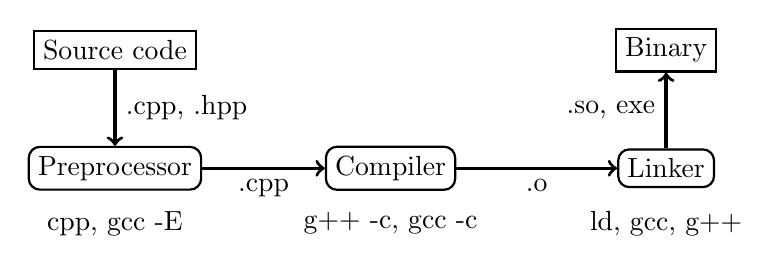
\begin{tikzpicture}
    \draw[thick] node (code) at(0,0) [rectangle,draw] {Source code}
                 node (cpp) at(0, -1.5cm) [rectangle,rounded corners,draw] {Preprocessor}
                 node (gcc) at(3.5cm,-1.5cm) [rectangle,rounded corners,draw] {Compiler}
                 node (ld) at(7cm,-1.5cm) [rectangle,rounded corners,draw] {Linker}
                 node (bin) at(7cm,0) [rectangle,draw] {Binary}
                 node at(0, -2.2cm) {cpp, gcc -E}
                 node at(3.5cm, -2.2cm) {g++ -c, gcc -c}
                 node at(7cm, -2.2cm) {ld, gcc, g++};
    \draw[very thick,->] (code) -- (cpp) node [midway,right] {.cpp, .hpp};
    \draw[very thick,->] (cpp) -- (gcc) node [midway,below] {.cpp};
    \draw[very thick,->] (gcc) -- (ld) node [midway,below] {.o};
    \draw[very thick,->] (ld) -- (bin) node [midway,left] {.so, exe};
  \end{tikzpicture}
  \begin{block}{The steps}
    \begin{description}
    \item[cpp]
        the preprocessor \\
        handles the \# directives (macros, includes) \\
        creates ``complete'' source code
    \item[g++]
        the compiler \\
        creates assembly code from \cpp code
    \item[ld]
        the linker \\
        links several binary files into libraries and executables
    \end{description}
  \end{block}
\end{frame}

\begin{frame}[fragile]
  \frametitle{Compilers}
  \begin{block}{Available tools}
    \begin{description}
    \item[\href{http://gcc.gnu.org/}{\beamergotobutton{gcc}}]
        the most common and most used\\
        free and open source
    \item[\href{http://clang.llvm.org/}{\beamergotobutton{clang}}]
        drop-in replacement of gcc \\
        better output and error reporting \\
        free and open source
    \item[\href{http://software.intel.com/en-us/intel-compilers}{\beamergotobutton{icc}}]
        the intel compiler \\
        proprietary \\
        optimized for Intel hardware
    \item[\href{http://www.microsoft.com/}{\beamergotobutton{Visual \cpp}}]
      the Windows way
    \end{description}
  \end{block}
  \begin{alertblock}{My prefered choice today}
    \begin{itemize}
      \item \hspace{0pt}\alert{clang} for its error reporting
      \item \alert{gcc} is not far and tries to catch up
    \end{itemize}
  \end{alertblock}
\end{frame}

\begin{frame}[fragile]
  \frametitle{Useful compiler options (gcc/clang)}
  \begin{block}{Get more warnings}
    \begin{description}
      \item[-Wall -Wextra] the way to get all warnings
      \item[-Werror] the way to force yourself to look at warnings
    \end{description}
  \end{block}
  \begin{block}{Around optimization}
    \begin{description}
      \item[-g] add debug symbols
      \item[-O0, -O2] 0 = no optimization, -O2 = optimized
    \end{description}
  \end{block}
  \begin{block}{Compilation environment}
    \begin{description}
      \item[\texttt{-I} \textless{}path\textgreater] where to find header files
      \item[\texttt{-L} \textless{}path\textgreater] where to find libraries
      \item[\texttt{-l} \textless{}name\textgreater] link with libname.so
      \item[\texttt{-E / -c}] stop after preprocessing / compilation
    \end{description}
  \end{block}
\end{frame}

\begin{frame}[fragile]
  \frametitle{Makefiles}
  \begin{block}{Why to use them}
    \begin{itemize}
    \item an organized way of describing building steps
    \item avoids a lot of typing
    \end{itemize}
  \end{block}
  \begin{block}{Several implementations}
    \begin{itemize}
    \item raw Makefiles : suitable for small projects
    \item cmake : portable, the current best choice
    \item automake : portable but complex
      \end{itemize}
  \end{block}
  \begin{minted}{makefile}
    test : test.cpp libpoly.so
        $(CXX) -Wall -Wextra -o $@ $^
    libpoly.so: Polygons.cpp
        $(CXX) -Wall -Wextra -shared -fPIC -o $@ $^
    clean:
        rm -f *o *so *~ test test.sol
  \end{minted}
\end{frame}

\begin{frame}[fragile]
  \frametitle{Compiler chain}
  \begin{alertblock}{Exercise Time}
    \begin{itemize}
    \item go to code/polymorphism
    \item preprocess Polygons.cpp (cpp or gcc -E -o output)
    \item compile Polygons.o and test.o (g++ -c -o output)
    \item use nm to check symbols
    \item see link statement using g++ -v
    \item see library dependencies with ldd
    \item look at the Makefile
    \item try make clean; make
    \end{itemize}
  \end{alertblock}
\end{frame}

\subsection[gdb]{Debugging}

\begin{frame}[fragile]
  \frametitle{Debugging}
  \begin{alertblock}{The problem}
    \begin{itemize}
      \item everything compiles fine (no warning)
      \item but crashes at run time
      \item no error message, no clue
    \end{itemize}
  \end{alertblock}
  \pause
  \begin{block}{The solution : debuggers}
    \begin{itemize}
    \item dedicated program able to stop execution at any time
    \item and show you where you are and what you have
    \end{itemize}
  \end{block}
  \pause
  \begin{block}{Existing tools}
    \begin{description}
    \item[\href{http://www.sourceware.org/gdb/}{\beamergotobutton{gdb}}]
      THE main player
    \item[\href{http://lldb.llvm.org/}{\beamergotobutton{lldb}}]
      the debugger coming with clang \\
      still young, no stable version
    \item[\href{http://software.intel.com/en-us/articles/idb-linux}{\beamergotobutton{idb}}]
      the intel debugger, proprietary
    \end{description}
  \end{block}
\end{frame}

\begin{frame}[fragile]
  \frametitle{gdb crash course}
  \begin{block}{start gdb}
    \begin{itemize}
    \item gdb \textless{}program\textgreater
    \item gdb \textless{}program\textgreater \textless{}core file\textgreater
    \end{itemize}
  \end{block}
  \begin{block}{inspect state}
    \begin{description}
    \item[bt] prints a backtrace
    \item[print \textless{}var\textgreater] prints current content of the variable
    \item[list] show code around current point
    \item[up/down] go up or down in call stack
    \end{description}
  \end{block}
  \begin{block}{breakpoints}
    \begin{description}
    \item[break \textless{}function\textgreater] puts a breakpoint on function entry
    \item[break \textless{}file\textgreater:\textless{}line\textgreater] puts a breakpoint on that line
    \end{description}
  \end{block}
\end{frame}

\begin{frame}[fragile]
  \frametitle{gdb}
  \begin{alertblock}{Exercise Time}
    \begin{itemize}
    \item go to code/debug
    \item compile, run, see the crash
    \item run it in gdb
    \item inspect backtrace, variables
    \item find problem and fix bug
    \item try stepping, breakpoints
    \item use -Wall -Wextra and see warning
    \end{itemize}
  \end{alertblock}
\end{frame}

\subsection[valgrind]{The Valgrind family}

\begin{frame}[fragile]
  \frametitle{The valgrind family}
  \begin{block}{Valgrind fundamentals}
    \begin{itemize}
    \item valgrind is a framework for different tools
    \item a processor simulator allowing checks in between instructions
    \item slow (10-50 times slower than normal execution)
    \item easy to use : ``valgrind \textless{}your executable\textgreater''
      \begin{itemize}
      \item no recompilation
      \item better with -g -O0, but not strictly needed
      \end{itemize}
    \item it is free and open source
    \end{itemize}
  \end{block}
  \pause
  \begin{block}{Main tools}
    \begin{description}
      \item[memcheck] a memory checker (default tool) and leak detector
      \item[callgrind] a call graph builder
      \item[helgrind] a race condition detector
    \end{description}
  \end{block}
\end{frame}

\begin{frame}[fragile]
  \frametitle{memcheck}
  \begin{block}{}
    \begin{itemize}
      \item keeps track of all memory allocations and deallocations
      \item is able to detect accesses to non allocated memory
      \item and even tell you when it was deallocated if it was
      \item or what it the closest array in case of overflow
      \item is able to list still allocated memory when program exits\\
        (memory leaks detection)
    \end{itemize}
  \end{block}
\end{frame}

\begin{frame}[fragile]
  \frametitle{valgrind}
  \begin{alertblock}{Exercise Time}
    \begin{itemize}
    \item go to code/valgrind
    \item compile, run, it should work
    \item run with valgrind, see the problem
    \item fix the problem
      \vspace{.3cm}
    \item go back to the code/debug exercise
    \item check it with valgrind
    \item analyze the issue, see that the variance was biaised
    \item fix the issue
    \end{itemize}
  \end{alertblock}
\end{frame}

\begin{frame}[fragile]
  \frametitle{memcheck}
  \begin{alertblock}{Exercise Time}
    \begin{itemize}
    \item go to code/memcheck
    \item compile, run, it should work
    \item run with valgrind, see LEAK summary
    \item run with -{}-leak-check=full to get details
    \item analyze and correct it
    \end{itemize}
  \end{alertblock}
\end{frame}

\begin{frame}[fragile]
  \frametitle{callgrind and kcachegrind}
  \begin{block}{callgrind}
    \begin{itemize}
      \item keeps track of all function calls
      \item and time spent in each function
      \item build statistics on calls, CPU usages and more
      \item outputs flat statistics file, quite unreadable
    \end{itemize}
  \end{block}
  \begin{block}{kcachegrind}
    \begin{itemize}
      \item a gui exploiting statistics built by callgrind
      \item able to browse graphically the program calls
      \item able to ``graph'' CPU usage on the program structure
    \end{itemize}
  \end{block}
\end{frame}

\begin{frame}[fragile]
  \frametitle{callgrind}
  \begin{alertblock}{Exercise Time}
    \begin{itemize}
    \item go to code/callgrind
    \item compile, run, it will be slow
    \item change nb iterations to 20
    \item run with valgrind -{}-tool=callgrind
    \item look at output with kcachegrind
    \item change fibo call to fibo2
    \item observe the change in kcachegrind
    \end{itemize}
  \end{alertblock}
\end{frame}

\begin{frame}[fragile]
  \frametitle{helgrind}
  \begin{block}{}
    \begin{itemize}
      \item keeps track of all pthreads activity
      \item in particular keeps track of all mutexes
      \item builds a graph of dependencies of the different actions
      \item works on the resulting graph to detect:
        \begin{itemize}
        \item possible dead locks
        \item possible data races
        \end{itemize}
    \end{itemize}
  \end{block}
  \pause
  \begin{alertblock}{}
    Note the ``possible''. It finds future problems !
  \end{alertblock}
\end{frame}

\begin{frame}[fragile]
  \frametitle{helgrind}
  \begin{alertblock}{Exercise Time}
    \begin{itemize}
    \item go to code/helgrind
    \item compile, run
    \item check it with valgrind. See strange behavior \\
      but no explanation
    \item check it with valgrind -{}-tool=helgrind
    \item understand issue and fix
    \end{itemize}
  \end{alertblock}
\end{frame}

\subsection[static]{Static code analysis}

\begin{frame}[fragile]
  \frametitle{Static analysis}
  \begin{alertblock}{The problem}
    \begin{itemize}
    \item all the tools discussed so far work on binaries
    \item they analyze the code being run
    \item so there is a coverage problem (e.g. for error cases)
    \end{itemize}
  \end{alertblock}
  \pause
  \begin{block}{A (partial) solution : analyzing the source code}
    \begin{itemize}
    \item build a graph of dependencies of the calls
    \item use graph tools to detect potential memory corruptions,
      memory leaks ot missing initializations
    \end{itemize}
  \end{block}
  \pause
  \begin{block}{Existing tools}
    \begin{description}
    \item[\href{http://www.coverity.com/}{\beamergotobutton{Coverity}}]
      proprietary tool, the most complete
    \item[\href{http://cppcheck.sourceforge.net/}{\beamergotobutton{cppcheck}}]
      free and opensource, but less complete
    \item[\href{http://clang-analyzer.llvm.org/}{\beamergotobutton{scan-build}}]
      the clang source analyzer, still young
    \end{description}
  \end{block}
\end{frame}

\begin{frame}[fragile]
  \frametitle{cppcheck}
  \begin{alertblock}{Exercise Time}
    \begin{itemize}
    \item go to code/cppcheck
    \item compile, run, see that it works
    \item use valgrind : no issue
    \item use cppcheck, see the problem
    \item analyze the issue, and fix it
    \item bonus : understand why valgrind did not complain \\
      and how the standard deviation could be biased \\
      hint : use gdb and check addresses of v and diffs
    \end{itemize}
  \end{alertblock}
\end{frame}

\section[conc]{Concurrency}

\subsection[thr]{Threads and async}

\begin{frame}[fragile]
  \frametitleii{Basic concurrency}
  \begin{block}{Threading}
    \begin{itemize}
    \item new object std::thread in \textless{}thread\textgreater{} header
    \item takes a function as argument of its constructor
    \item must be detached or joined before the main thread terminates
    \item \cpp20: std::jthread automatically joins at destruction
    \end{itemize}
  \end{block}
  \pause
  \begin{exampleblock}{Example code}
    \begin{cppcode*}{}
      void doSth() {...}
      void doSthElse() {...}
      int main() {
        std::thread t1(doSth);
        std::thread t2(doSthElse);
        for (auto t: {&t1,&t2}) t->join();
      }
    \end{cppcode*}
  \end{exampleblock}
\end{frame}

\begin{frame}[fragile]
  \frametitleii{The thread constructor}
  \begin{exampleblock}{Can take a function and its arguments}
    \begin{cppcode*}{}
      void function(int j, double j) {...};
      std::thread t1(function, 1, 2.0);
    \end{cppcode*}
  \end{exampleblock}
  \pause
  \begin{exampleblock}{Can take any function-like object}
    \begin{cppcode*}{}
      struct AdderFunctor {
        AdderFunctor(int i): m_i(i) {}
        int operator() (int j) { return i+j; };
        int m_i;
      };
      std::thread t2(AdderFunctor(2), 5);
      int a;
      std::thread t3([](int i) { return i+2; }, a);
      std::thread t4([a]       { return a+2; });
    \end{cppcode*}
  \end{exampleblock}
\end{frame}

\begin{frame}[fragile]
  \frametitleii{Basic asynchronicity}
  \begin{block}{Concept}
    \begin{itemize}
    \item separation of the specification of what should be done and the retrieval of the results
    \item ``start working on this, and ping me when it's ready''
    \end{itemize}
  \end{block}
  \pause
  \begin{block}{Practically}
    \begin{itemize}
    \item std::async function launches an asynchronous task
    \item std::future template allows to handle the result
    \end{itemize}
  \end{block}
  \pause
  \begin{exampleblock}{Example code}
    \begin{cppcode*}{}
      int computeSth() {...}
      std::future<int> res = std::async(computeSth);
      std::cout << res->get() << std::endl;
    \end{cppcode*}
  \end{exampleblock}
\end{frame}

\begin{frame}[fragile]
  \frametitleii{Mixing the two}
  \begin{block}{Is async running concurrent code ?}
    \begin{itemize}
    \item it depends !
    \item you can control this with a launch policy argument
      \begin{description}
      \item[std::launch::async] spawns a thread for immediate execution
      \item[std::launch::deferred] causes lazy execution in current thread
      \end{description}
      \begin{itemize}
      \item execution starts when get() is called
      \end{itemize}
    \item default is not specified !
    \end{itemize}
  \end{block}
  \pause
  \begin{exampleblock}{Usage}
    \begin{cppcode*}{}
      int computeSth() {...}
      auto res = std::async(std::launch::async,
                            computeSth);
      auto res2 = std::async(std::launch::deferred,
                             computeSth);
    \end{cppcode*}
  \end{exampleblock}
\end{frame}

\begin{frame}[fragile]
  \frametitleii{Fine grained control on asynchronous execution}
  \begin{block}{std::packaged\_task template}
    \begin{itemize}
    \item creates an asynchronous version of any function-like object
      \begin{itemize}
      \item identical arguments
      \item returns a std::future
      \end{itemize}
    \item provides access to the returned future
    \item associated with threads, gives full control on execution
    \end{itemize}
  \end{block}
  \pause
  \begin{exampleblock}{Usage}
    \begin{cppcode*}{}
      int task() { return 42; }
      std::packaged_task<int()> pckd_task(task);
      auto future = pckd_task.get_future();
      pckd_task();
      std::cout << future.get() << std::endl;
    \end{cppcode*}
  \end{exampleblock}
\end{frame}

\subsection[mutex]{Mutexes}

\begin{frame}[fragile]
  \frametitleii{Races}
  \begin{exampleblock}{Example code}
    \begin{cppcode*}{}
      int a = 0;
      void inc() { a++; };
      void inc100() {
        for (int i=0; i < 100; i++) inc();
      };
      int main() {
        std::thread t1(inc100);
        std::thread t2(inc100);
        for (auto t: {&t1,&t2}) t->join();
        std::cout << a << std::endl;
      }
    \end{cppcode*}
  \end{exampleblock}
  \pause
  \begin{block}{What do you expect ? Try it in code/race}
    \pause
    Anything between 100 and 200 !!!
  \end{block}
\end{frame}

\begin{frame}[fragile]
  \frametitleii{Atomicity}
  \begin{exampleblock}{Definition (wikipedia)}
    \begin{itemize}
    \item an operation (or set of operations) is atomic if it appears to the rest of the system to occur instantaneously
    \end{itemize}
  \end{exampleblock}
  \begin{block}{Practically}
    \begin{itemize}
    \item an operation that won't run concurrently to another one
    \item an operation that will have a stable environment during execution
    \end{itemize}
  \end{block}
  \pause
  \begin{alertblock}{Is ++ operator atomic ?}
    \pause
    Usually not. It behaves like :
    \begin{cppcode*}{}
      eax = a       // memory to register copy
      increase eax  // increase (atomic CPU instruction)
      a = eax       // copy back to memory
    \end{cppcode*}
  \end{alertblock}
\end{frame}

\begin{frame}[fragile]
  \frametitleii{Timing}
  \begin{exampleblock}{Code}
    \begin{cppcode*}{}
      eax = a       // memory to register copy
      increase eax  // increase (atomic CPU instruction)
      a = eax       // copy back to memory
    \end{cppcode*}
  \end{exampleblock}
  \begin{block}{For 2 threads}
    \begin{tikzpicture}
      \begin{umlseqdiag}
        \umlobject[x=0, class=eax]{Thread 1}
        \umlobject[x=3, class=a, fill=blue!20]{Memory}
        \umlobject[x=6, class=eax]{Thread 2}
        \begin{umlcall}[op=read, type=synchron, return=0]{Thread 1}{Memory}
        \end{umlcall}
        \begin{umlcall}[padding=3, op=read, type=synchron, return=0]{Thread 2}{Memory}
        \end{umlcall}
        \begin{umlcallself}[op=incr, type=synchron]{Thread 1}
        \end{umlcallself}
        \begin{umlcallself}[op=incr, type=synchron]{Thread 2}
        \end{umlcallself}
        \begin{umlcall}[op=write 1]{Thread 2}{Memory}
        \end{umlcall}
        \begin{umlcall}[padding=3, op=write 1]{Thread 1}{Memory}
        \end{umlcall}
      \end{umlseqdiag}
      \draw[-triangle 60](8.5,0) -- (8.5,-4) node[right, pos=0.5]{time};
    \end{tikzpicture}
  \end{block}
\end{frame}

\begin{frame}[fragile]
  \frametitleii{Mutexes}
  \begin{block}{Concept}
    \begin{itemize}
    \item a lock to serialize access to a non-atomic piece of code
    \end{itemize}
  \end{block}
  \pause
  \begin{block}{The objects}
    \begin{description}[labelwidth=1.8cm]
    \item[std::mutex] in the mutex header
    \item[std::lock\_guard] for an RAII version of it
    \item[std::unique\_lock] same and can be released/relocked
    \end{description}
  \end{block}
  \pause
  \begin{exampleblock}{Practically}
    \begin{cppcode*}{}
      int a = 0;
      std::mutex m;
      void inc() {
        std::lock_guard<std::mutex> guard(m);
        a++;
      };
    \end{cppcode*}
  \end{exampleblock}
\end{frame}

\begin{frame}[fragile]
  \frametitleii{Mutexes}
  \begin{alertblock}{Exercise Time}
    \begin{itemize}
    \item Go to code/race
    \item Look at the code and try it\\
      See that it has a race condition
    \item Use a mutex to fix the issue
    \item See the difference in execution time
    \end{itemize}
  \end{alertblock}
\end{frame}

\begin{frame}[fragile]
  \frametitleii{Dead lock}
  \begin{exampleblock}{Scenario}
    \begin{itemize}
    \item 2 mutexes, 2 threads
    \item locking order different in the 2 threads
    \end{itemize}
  \end{exampleblock}
  \pause
  \begin{block}{Sequence diagram}
    \begin{tikzpicture}
      \begin{umlseqdiag}
        \umlobject[x=0]{Thread 1}
        \umlobject[x=2.5, fill=blue!20]{Mutex A}
        \umlobject[x=5, fill=blue!20]{Mutex B}
        \umlobject[x=7.5]{Thread 2}
        \begin{umlcall}[op=lock]{Thread 1}{Mutex A}
        \end{umlcall}
        \begin{umlcall}[op=lock, dt=6]{Thread 2}{Mutex B}
        \end{umlcall}
        \begin{umlcall}[op=lock (block), dt=6]{Thread 1}{Mutex B}
        \end{umlcall}
        \begin{umlcall}[op=lock (block), dt=12]{Thread 2}{Mutex A}
        \end{umlcall}
      \end{umlseqdiag}
      \draw[-triangle 60](9,0) -- (9,-4) node[right, pos=0.5]{time};
    \end{tikzpicture}
  \end{block}
\end{frame}

\begin{frame}[fragile]
  \frametitleii{How to avoid dead locks}
  \begin{block}{Possible solutions}
    \begin{itemize}
    \item Never take several locks
      \begin{itemize}
      \item Or add master lock protecting the locking phase
      \end{itemize}
    \item Respect a strict order in the locking across all threads
    \item Do not use locks
      \begin{itemize}
      \item Use other techniques, e.g. queues
      \end{itemize}
    \end{itemize}
  \end{block}
\end{frame}

\begin{frame}[fragile]
  \frametitleii{Condition variables}
  \begin{block}{How to express thread dependencies}
    \begin{itemize}
    \item Allows a thread to sleep until a given condition is satisfied
    \item std::condition\_variable object from condition\_variable header
    \end{itemize}
  \end{block}
  \pause
  \begin{block}{Usage}
    \begin{itemize}
    \item wraps an RAII lock around a mutex
    \item wait() will hang until the condition is met
      \begin{itemize}
      \item you can have several waiters sharing the same mutex
      \end{itemize}
    \item notify\_one() will wake up one waiter
    \item notify\_all() will wake up all waiters
    \end{itemize}
  \end{block}
\end{frame}

\begin{frame}[fragile]
  \frametitleii{Condition variable usage}
  \begin{exampleblock}{Example code}
    \begin{cppcode*}{}
      int value = -1;
      std::mutex mutex;
      std::condition_variable cond;
      auto t1 = std::thread([&cond] () {
        value = ... long process ...;
        cond.notify_all();
      });
      auto t2 = std::thread([&cond,&mutex,&value] () {
        std::unique_lock<std::mutex> lock{mutex};
        cond.wait(lock, [&value] { return value > 0; });
        ... use value ...
      });
      { std::unique_lock<std::mutex> lock{mutex};
        cond.wait(lock, [] { return value > 0; });
        std::cout << value << std::endl; }
    \end{cppcode*}
  \end{exampleblock}
\end{frame}



\section[py]{\cpp and python}

\subsection[module]{Writing a module}

\begin{frame}[fragile]
  \frametitle{How to build a python 3 module around \cpp code}
  \begin{block}{\cpp code : mandel.hpp}
    \begin{cppcode*}{}
      int mandel(Complex const & a);
    \end{cppcode*}
  \end{block}
\end{frame}

\begin{frame}[fragile]
  \frametitle{Basic Module(1) : wrap your method}
  \begin{block}{mandelModule.cpp - see code/python exercise}
    \begin{cppcode*}{}
      #include <Python.h>
      #include "mandel.hpp"
      PyObject * mandel_wrapper(PyObject * self,
                                PyObject * args) {
        // Parse Input
        float r, i;
        if (!PyArg_ParseTuple(args, "ff", &r, &i))
          return NULL;
        // Call C++ function
        int result = mandel(Complex(r, i));
        // Build returned objects
        return PyLong_FromLong(result);
      }
    \end{cppcode*}
  \end{block}
\end{frame}

\begin{frame}[fragile]
  \frametitle{Basic Module(2) : create the python module}
  \begin{block}{mandelModule.cpp - see code/python exercise}
    \begin{cppcode*}{}
      // declare the modules' methods
      PyMethodDef mandelMethods[] = {
          {"mandel", mandel_wrapper, METH_VARARGS,
          "computes nb of iterations for mandelbrot set"},
          {NULL, NULL, 0, NULL}
      };
      // declare the module
      struct PyModuleDef mandelModule = {
        PyModuleDef_HEAD_INIT,
        "mandel", NULL, -1, mandelMethods
      };
      PyMODINIT_FUNC PyInit_mandel(void) {
        return PyModule_Create(&mandelModule);
      }
    \end{cppcode*}
  \end{block}
\end{frame}

\begin{frame}[fragile]
  \frametitle{Basic Module(3) : use it}
  \begin{block}{First compile the module}
    \begin{itemize}
    \item as a regular shared library
    \item with '-I \$(PYTHON\_INCLUDE)'
    \end{itemize}
  \end{block}
  \begin{block}{mandel.py - see code/python exercise}
    \begin{minted}[gobble=4]{python}
      from mandel import mandel
      v = mandel(0.7, 1.2)
    \end{minted}
  \end{block}
\end{frame}


\subsection[C]{Marrying \cpp and C}

\begin{frame}[fragile]
  \frametitle{A question of mangling}
  \begin{block}{Mangling}
    the act of converting the name of variable or function to a symbol name in the binary code
  \end{block}
  \begin{block}{C versus \cpp symbol names}
    \begin{itemize}
    \item C uses bare function name
    \item \cpp allows overloading of functions by taking the signature into account
    \item so \cpp mangling has to contain signature
    \end{itemize}
  \end{block}
\end{frame}

\begin{frame}[fragile]
  \frametitle{C mangling}
  \begin{exampleblock}{Source : file.c}
    \begin{cppcode*}{}
      float sum(float a, float b);
      int square(int a);
      // won't compile : conflicting types for ‘square’
      // float square(float a);
    \end{cppcode*}
  \end{exampleblock}
  \begin{block}{Binary symbols : file.o}
    \begin{minted}[gobble=4]{shell}
      # nm file.o
      000000000000001a T square
      0000000000000000 T sum
    \end{minted}
  \end{block}
\end{frame}

\begin{frame}[fragile]
  \frametitle{\cpp mangling}
  \begin{exampleblock}{Source : file.cpp}
    \begin{cppcode*}{}
      float sum(float a, float b);
      int square(int a);
      // ok, signature is different
      float square(float a);
    \end{cppcode*}
  \end{exampleblock}
  \begin{block}{Binary symbols : file.o}
    \begin{minted}[gobble=4]{shell}
      # nm file.o
      0000000000000000 T _Z3sumff
      000000000000002a T _Z6squaref
      000000000000001a T _Z6squarei
    \end{minted}
  \end{block}
\end{frame}

\begin{frame}[fragile]
  \frametitle{Forcing C mangling in \cpp}
  \begin{block}{extern ``C''}
    These functions will use C mangling :
    \begin{cppcode*}{gobble=1}
      extern "C" {
        float sum(float a, float b);
        int square(int a);
      }
    \end{cppcode*}
  \end{block}
  \pause
  You can now call these \cpp functions from C code
  \pause
  \begin{alertblock}{Limitations}
    \begin{itemize}
    \item no \cpp types should go out
    \item no exceptions either (use noexcept here)
    \item member functions cannot be used
      \begin{itemize}
      \item they need to be wrapped one by one
      \end{itemize}
    \end{itemize}
  \end{alertblock}
\end{frame}

\subsection[ctypes]{The ctypes module}

\begin{frame}[fragile]
  \frametitle{The ctypes python module}
  \begin{block}{From the documentation}
    \begin{itemize}
    \item provides C compatible data types
    \item allows calling functions in DLLs or shared libraries
    \item can be used to wrap these libraries in pure Python
    \end{itemize}
  \end{block}
\end{frame}

\begin{frame}[fragile]
  \frametitle{ctypes : usage example}
  \begin{block}{\cpp code : mandel.hpp}
    \begin{cppcode*}{}
      int mandel(Complex const & a);
    \end{cppcode*}
  \end{block}
  \begin{block}{``C'' code : mandel\_cwrapper.hpp}
    \begin{cppcode*}{}
      extern "C" {
        int mandel(float r, float i) {
          return mandel(Complex(r, i));
        };
      }
    \end{cppcode*}
  \end{block}
  \begin{exampleblock}{calling the mandel library}
    \begin{minted}[gobble=4]{python}
      from ctypes import *
      libmandel = CDLL('libmandelc.so')
      v = libmandel.mandel(c_float(0.3), c_float(1.2))
    \end{minted}
  \end{exampleblock}
\end{frame}

\begin{frame}
  \frametitle{Marrying \cpp and python}
  \begin{alertblock}{Exercise Time}
    \begin{itemize}
    \item go to code/python
    \item look at the original python code mandel.py
    \item time it (`time python3 mandel.py`)
    \item look at the code in mandel.hpp/cpp
    \item look at the python module mandel\_module.cpp
    \item compile and modify mandel.py to use it
    \item see the gain in time
    \item look at the C wrapper in mandel\_cwrapper.cpp
    \item modify mandel.py to use libmandelc directly with ctypes
    \end{itemize}
  \end{alertblock}
  \tiny Note : you may have to add '.' to LD\_LIBRARY\_PATH and PYTHONPATH
\end{frame}

\subsection[cppyy]{The cppyy project}

\begin{frame}
  \frametitle{Automatic Python-C++ bindings}
  \begin{block}{The {\color{blue!50!white} \href{https://cppyy.readthedocs.io}{cppyy}} project}
    \begin{itemize}
    \item originated from the ROOT project
    \item still young, version 1.0 from Mid 2018
    \item but very active,  current version 2.1.0
    \item extremely powerful for interfacing \cpp and python
    \end{itemize}
  \end{block}
  \begin{block}{How it works}
    \begin{itemize}
    \item uses Just in Time compilation through {\color{blue!50!black} \href{https://github.com/vgvassilev/cling}{cling}}
      \begin{itemize}
      \item an interactive \cpp interpreter
      \end{itemize}
    \end{itemize}
  \end{block}
\end{frame}

\begin{frame}
  \frametitle{cppyy crash course(1)}
  Shamelessly copied from the cppyy documentation
  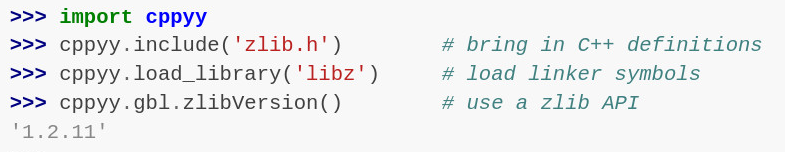
\includegraphics[width=.8\textwidth]{python/cppyy2.png}
  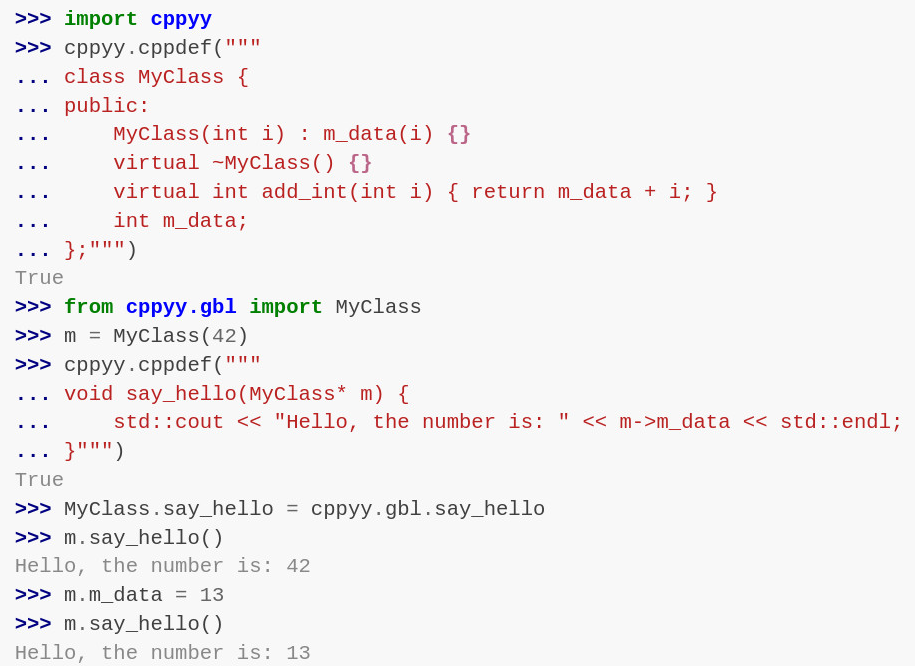
\includegraphics[trim={0 3.2cm 0 0},clip,width=\textwidth]{python/cppyy.png}
\end{frame}

\begin{frame}
  \frametitle{cppyy crash course(1)}
  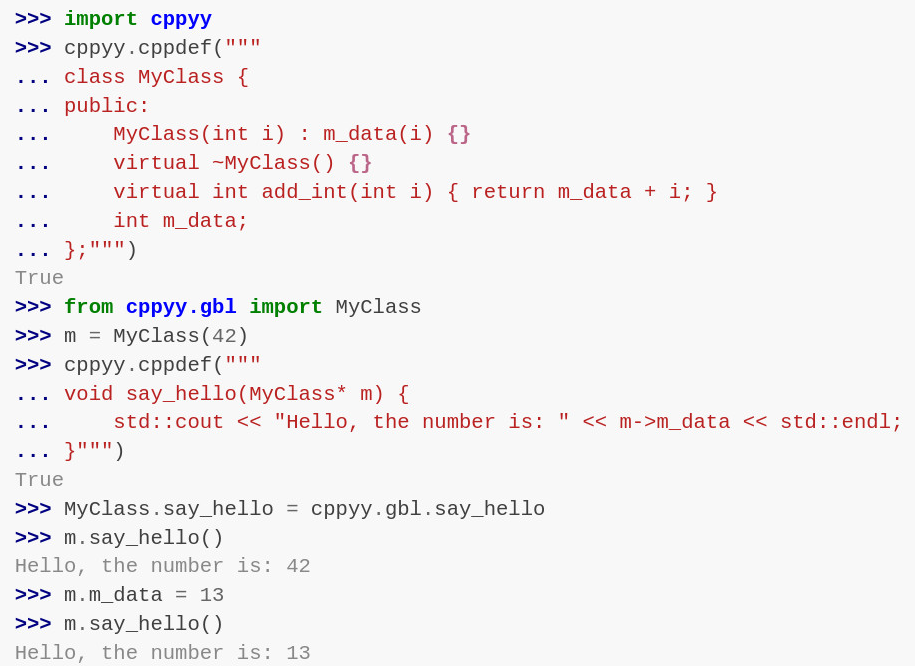
\includegraphics[trim={0 0 0 2.45cm},clip,width=\textwidth]{python/cppyy.png}
\end{frame}


\begin{frame}
  \frametitle{This is the end}
  \begin{center}
    \Huge Questions ?\\
    \vspace{.5cm}
    \tiny \href{https://github.com/hsf-training/cpluspluscourse}{https://github.com/hsf-training/cpluspluscourse}\\
    \tiny \href{http://cern.ch/sponce/C++Course}{http://cern.ch/sponce/C++Course}
  \end{center}
\end{frame}

\end{document}
